\chapter{Hamilton--Jacobi方程}
\label{chap:hamilton-jacobi-equations}

一个波前从一点出发，以当地的速度向四周推进。对平面上的每个位置，最早什么时候被波前扫到？把这个时刻记成函数$T(\bm{x})$。沿着波前的法向走一小步，所花时间等于步长除以当地速度，于是$T$的梯度长度由速度决定。这条关系对未知函数的梯度是非线性的：两个解的和不再是解。

求解$T$并不需要把波前一步步推进。在解光滑的地方，$T$可以沿一族曲线算出来，这些曲线就是波前的传播路线。麻烦出现在路线相交的地方。两列波前相遇时，一个位置会被两条路线同时到达，两条路线给出不同的梯度，$T$在那里长出尖点。路线之后还能继续画，算出的值却不止一个，而物理上只有第一次到达才算数。

本章先建立两类问题：到达时间的边值问题和随时间演化的初值问题，并说清Hamilton量在其中的作用。接着用特征线在光滑的范围内重建解，再看尖点怎样产生，为什么“几乎处处满足方程”不足以确定解。然后在接触点处提出微分不等式，得到黏性解的定义，由比较原理证明唯一性和数据稳定性。最后讨论两种得到解的办法：Hopf--Lax公式把解写成极小化，消失黏性把解看成小扩散方程的极限。这两种办法与尖点处的选择完全一致。

\section{方程问题}
\label{sec:hj-problem}

先把两类问题摆出来。一类问波前什么时候到达，未知函数不含时间；另一类问一个高度场随时间怎样变化，它的变化率由局部斜率决定。前者可以看成后者的特例，两者需要的数据却不一样。

\paragraph{到达时间}
从一维开始。在$x=0$处点火，火线以速度$c(x)>0$向右推进。经过一小段$[x,x+\mathrm{d}x]$需要的时间是$\mathrm{d}x/c(x)$，把这些时间加起来得到到达时间
\[
  T(x)=\int_0^x\frac{\mathrm{d}s}{c(s)},\qquad T'(x)=\frac{1}{c(x)}.
\]
速度越小，到达时间增长得越快，$T$的斜率就是“慢度”$1/c$。

取一组具体的速度：在$[0,1)$上$c=1$，在$[1,2)$上$c=0.4$，在$[2,3]$上$c=1.5$。逐段累加，得到
\[
  T(1)=1,\qquad T(2)=1+\frac{1}{0.4}=3.5,\qquad T(3)=3.5+\frac{1}{1.5}\approx4.17.
\]
图~\ref{fig:hj-arrival-1d}显示，$T$是折线，慢的中间一段最陡。

\begin{BookInlineFigure}
  \centering
  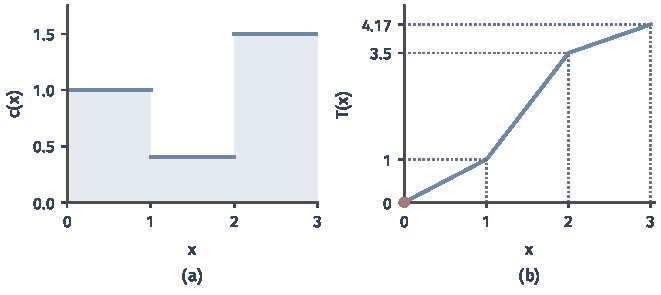
\includegraphics[width=112mm]{figures/06-differential-equations/02-partial-differential-equations/matplotlib/hj-arrival-1d/figure.pdf}
  \caption{一维到达时间。(a)分段常数的速度$c(x)$。(b)由$x=0$（红点）出发的到达时间$T(x)$，各段斜率是$1/c$。}
  \label{fig:hj-arrival-1d}
\end{BookInlineFigure}

到了高维，时刻$t$的波前是等值面$\{T=t\}$，已经被扫过的区域是$\{T\leq t\}$。设波前沿法向以速度$c(\bm{x})$推进。图~\ref{fig:hj-front-normal}中，点$\bm{x}$在$\mathrm{d}t$后沿法向$\bm{n}$到达$\bm{x}+c\,\mathrm{d}t\,\bm{n}$，那里的到达时间恰好多了$\mathrm{d}t$，所以
\[
  \langle\nabla T,\ c\,\bm{n}\rangle\,\mathrm{d}t=\mathrm{d}t.
\]
法向是$T$增长的方向，$\bm{n}=\nabla T/\lVert\nabla T\rVert_2$。代入后得到$c\,\lVert\nabla T\rVert_2=1$。

\begin{BookInlineFigure}
  \centering
  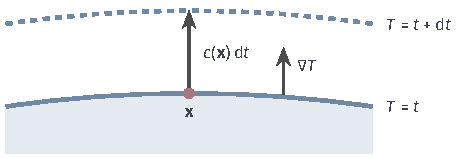
\includegraphics[width=78.3mm]{figures/06-differential-equations/02-partial-differential-equations/tikz/hj-front-normal/figure.pdf}
  \caption{波前的法向推进。实线是时刻$t$的波前，虚线是$t+\mathrm{d}t$的波前，浅蓝是已扫过的区域。两条等值线的法向距离是$c(\bm{x})\,\mathrm{d}t$，所以$\nabla T$的长度是$1/c$。}
  \label{fig:hj-front-normal}
\end{BookInlineFigure}

这个局部关系连同“从哪里开始、何时开始”的数据，构成到达时间问题。

\begin{definition}[程函方程]
\label{def:hj-eikonal}
设$\Omega\subset\mathbb{R}^{d}$是开集，$c:\Omega\to(0,\infty)$连续，$\Gamma\subset\overline{\Omega}$是闭集，$g:\Gamma\to\mathbb{R}$是给定的起始时刻。称
\begin{equation}
  c(\bm{x})\,\lVert\nabla T(\bm{x})\rVert_2=1\quad(\bm{x}\in\Omega\setminus\Gamma),\qquad
  T=g\quad\text{在}\ \Gamma\ \text{上}
  \label{eq:hj-eikonal}
\end{equation}
为\term{程函方程}（eikonal equation）的边值问题，$T$称为\term{到达时间}（arrival time），它的等值面$\{T=t\}$称为时刻$t$的\term{波前}（wavefront）。
\end{definition}

方程里没有时间，时间是未知函数的取值。一维时方程写作$\lvert T'\rvert=1/c$，比前面的$T'=1/c$少了方向信息：向左走还是向右走，方程本身不管。第~\ref{chap:pde-problems}章已经见过这种缺失带来的后果，$\lvert u'\rvert=1$、$u(\pm1)=0$没有$C^1$解，却有无穷多条几乎处处满足方程的锯齿线。

\paragraph{初值演化}
到达时间也可以放进一个随时间变化的场里。令$u(\bm{x},t)=T(\bm{x})-t$，则时刻$t$的波前就是$u(\cdot,t)$的零等值面。这时$\partial_tu=-1$，$\nabla u=\nabla T$，所以程函方程变成
\[
  \partial_tu+c(\bm{x})\,\lVert\nabla u\rVert_2=0.
\]
图~\ref{fig:hj-level-set}对$T(x)=\lvert x\rvert$画出这件事：函数图像整体下降，零点（红）就是向两侧跑的波前。

\begin{BookInlineFigure}
  \centering
  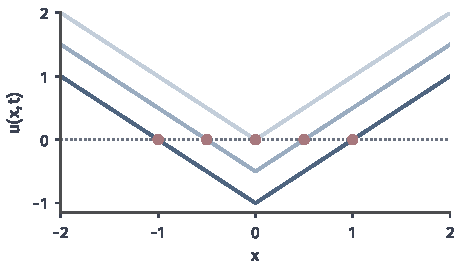
\includegraphics[width=78mm]{figures/06-differential-equations/02-partial-differential-equations/matplotlib/hj-level-set/figure.pdf}
  \caption{把波前写成零等值面。蓝色由浅到深是$u(x,t)=\lvert x\rvert-t$在$t=0,0.5,1$的图像，红点是零点$x=\pm t$，它们以速度$1$向两侧运动。}
  \label{fig:hj-level-set}
\end{BookInlineFigure}

把$c\lVert\bm{p}\rVert_2$换成一般的函数，就得到本章的第二类问题。

\begin{definition}[Hamilton--Jacobi初值问题]
\label{def:hj-ivp}
设$t_{\mathrm{f}}>0$，函数$H(t,\bm{x},\bm{p})$在$t\in[0,t_{\mathrm{f}}]$、$\bm{x},\bm{p}\in\mathbb{R}^{d}$上连续，$u_0$在$\mathbb{R}^{d}$上连续。称
\begin{equation}
  \partial_tu+H(t,\bm{x},\nabla u)=0\quad(\bm{x}\in\mathbb{R}^{d},\ 0<t<t_{\mathrm{f}}),\qquad
  u(\bm{x},0)=u_0(\bm{x})
  \label{eq:hj-ivp}
\end{equation}
为\term{Hamilton--Jacobi方程}（Hamilton--Jacobi equation）的初值问题，$H(t,\bm{x},\bm{p})$称为\term{Hamilton量}（Hamiltonian）。若$u$连续可微并逐点满足方程，就称$u$是经典解。
\end{definition}

本章的$u$只在$H$中通过梯度出现，$H$不依赖场值。比第~\ref{chap:transport-equations}章多出来的是：$H$对$\bm{p}$可以是非线性的。输运方程$\partial_tu+\langle\bm{v},\nabla u\rangle=0$正是$H=\langle\bm{v},\bm{p}\rangle$的线性情形。

\paragraph{Hamilton量的作用}
$H$回答的问题是：斜率为$\bm{p}$的地方，高度以多快的速度下降。这一点在平面解上能直接看出。对只依赖$\bm{p}$的$H$，令
\begin{equation}
  u(\bm{x},t)=\langle\bm{p},\bm{x}\rangle-tH(\bm{p}).
  \label{eq:hj-plane-solution}
\end{equation}
此时$\nabla u=\bm{p}$，$\partial_tu=-H(\bm{p})$，方程逐点成立。斜率不变，整个平面以速率$H(\bm{p})$下降。

图~\ref{fig:hj-plane-slopes}取$H(p)=p^2/2$。斜率$p=0,1,2$的三条直线在$t=1$时分别下降$0$、$0.5$和$2$。下降量对斜率是二次的。把两个斜率为$1$的解相加，得到的直线斜率为$2$，下降量却只有$1$，而斜率为$2$的解应当下降$2$，所以解不能叠加。

\begin{BookInlineFigure}
  \centering
  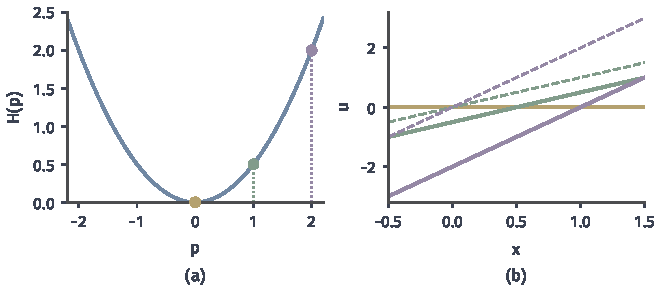
\includegraphics[width=112mm]{figures/06-differential-equations/02-partial-differential-equations/matplotlib/hj-plane-slopes/figure.pdf}
  \caption{Hamilton量决定下降速率。(a)$H(p)=p^2/2$，三个点对应$p=0,1,2$（黄、绿、紫）。(b)对应的平面解，虚线是$t=0$，实线是$t=1$，下降量分别是$0$、$0.5$、$2$。}
  \label{fig:hj-plane-slopes}
\end{BookInlineFigure}

一维时方程和第~\ref{chap:scalar-conservation-laws}章的守恒律有直接的关系。设$H=H(p)$，$u$足够光滑，对$\partial_tu+H(\partial_xu)=0$再求一次$x$偏导，$v=\partial_xu$满足
\[
  \partial_tv+\partial_xH(v)=0.
\]
所以一维的Hamilton--Jacobi方程是通量为$H$的标量守恒律的“原函数”，$u$的折角对应$v$的间断。这个对应后面会反复用到，但它只在一维成立；高维时梯度是向量，不满足标量守恒律。

\paragraph{两类问题需要的数据}
表~\ref{tab:hj-two-problems}把两类问题放在一起。两者都是对梯度的非线性方程，数据的位置和要求不同。

\begin{BookInlineTable}
  \centering
  \begin{tabular}{lll}
    \toprule
    & 到达时间问题 & 初值演化问题\\
    \midrule
    未知量 & $T(\bm{x})$，时间是取值 & $u(\bm{x},t)$\\
    梯度的含义 & 慢度向量，长度$1/c$ & 局部斜率\\
    方程的作用 & 限制梯度的长度 & 由斜率给出下降速率\\
    所需数据 & 源集合$\Gamma$上的起始时刻 & $t=0$时整个$\mathbb{R}^{d}$上的$u_0$\\
    数据的限制 & 起始时刻不能相互矛盾 & 增长和正则性\\
    \bottomrule
  \end{tabular}
  \caption{到达时间问题与初值演化问题的对比。}
  \label{tab:hj-two-problems}
\end{BookInlineTable}

初值问题只需要在$t=0$给一个函数，方程对时间是一阶的，不需要初始速度，全空间上也没有侧边界。到达时间问题的数据要彼此相容。在区间$(0,1)$上取$c=1$，两端都是源，起始时刻为$g(0)=0$和$g(1)=2$。从左端出发的波前在时刻$1$就到达了右端，而右端规定的起始时刻是$2$，这个规定不会起作用。一般的要求是，$\lvert g(\bm{x})-g(\bm{y})\rvert$不超过两点之间的传播时间；这个限制在第~\ref{sec:hj-comparison}节还要用到。

\section{特征方程}
\label{sec:hj-characteristics}

方程只说了时间导数和梯度的关系，能否沿某些曲线把它化成常微分方程？输运方程已经用过这个办法：沿速度场的轨线，解的值不变。这里的困难在于，方程对梯度非线性，沿曲线求导时会冒出二阶导数。这一节要找到让二阶导数消失的曲线，并说明怎样从这些曲线重建场。

\paragraph{沿什么曲线求导}
设$H$二阶连续可微，$u$是二阶连续可微的经典解。取一条待定的曲线$\bm{x}(s)$，记沿线的梯度和值为
\[
  \bm{p}(s)=\nabla u(\bm{x}(s),s),\qquad z(s)=u(\bm{x}(s),s).
\]
对$\bm{p}$求导，用链式法则，得到
\[
  \dot{\bm{p}}=\partial_t\nabla u+\nabla^2u\,\dot{\bm{x}}.
\]
这里出现了未知的二阶导数$\nabla^2u$，这是方程非线性的代价。

为消去$\partial_t\nabla u$，对方程本身关于$\bm{x}$求梯度：
\[
  \partial_t\nabla u+\nabla_{\bm{x}}H+\nabla^2u\,\nabla_{\bm{p}}H=0.
\]
两式相减消去$\partial_t\nabla u$，得到
\[
  \dot{\bm{p}}=-\nabla_{\bm{x}}H+\nabla^2u\,\bigl(\dot{\bm{x}}-\nabla_{\bm{p}}H\bigr).
\]
括号里的量可以由我们选择：只要曲线满足$\dot{\bm{x}}=\nabla_{\bm{p}}H$，二阶导数就消失了。曲线的方向不是事先给定的速度场，而由当地的斜率决定。

再算沿线的值。由链式法则和方程，
\[
  \dot{z}=\partial_tu+\langle\nabla u,\dot{\bm{x}}\rangle=-H+\langle\bm{p},\nabla_{\bm{p}}H\rangle.
\]
把这三个结果写在一起。

\begin{theorem}[特征方程组]
\label{thm:hj-characteristics}
设$H\in C^2$，$u\in C^2$是方程$\partial_tu+H(t,\bm{x},\nabla u)=0$的解。若曲线$\bm{x}(s)$的速度等于$\nabla_{\bm{p}}H$（梯度变量取沿线的$\nabla u$），则沿线的梯度$\bm{p}(s)$和值$z(s)$满足
\begin{equation}
  \dot{\bm{x}}=\nabla_{\bm{p}}H,\qquad
  \dot{\bm{p}}=-\nabla_{\bm{x}}H,\qquad
  \dot{z}=\langle\bm{p},\nabla_{\bm{p}}H\rangle-H,
  \label{eq:hj-characteristics}
\end{equation}
其中$H$及其偏导数都在$(s,\bm{x}(s),\bm{p}(s))$处取值。这组常微分方程称为\term{特征方程组}（characteristic system），$\bm{x}(s)$称为特征线。
\end{theorem}

式~\eqref{eq:hj-characteristics}的前两个方程不含$z$，构成$(\bm{x},\bm{p})$空间中的闭合系统，这就是第~\ref{chap:ode-sensitivity}章的Hamilton方程。在那里我们已经知道它生成的流保持相空间体积，$H$不显含时间时沿轨道守恒。这两条性质这里不再重复；本章的新内容是第三个方程，它在已知$(\bm{x},\bm{p})$之后只是一次积分，负责把值带上。

图~\ref{fig:hj-characteristic-lift}是一条特征线的示意。出发点$\bm{y}$提供初始斜率$\bm{p}_0=\nabla u_0(\bm{y})$，此后位置按$\nabla_{\bm{p}}H$前进，斜率按$-\nabla_{\bm{x}}H$变化，值按第三式累积。

\begin{BookInlineFigure}
  \centering
  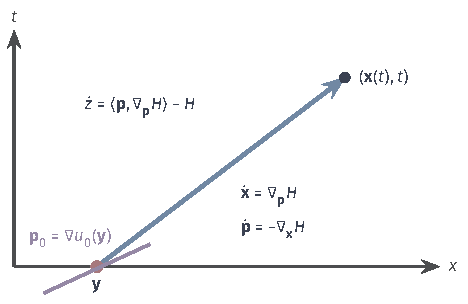
\includegraphics[width=79.3mm]{figures/06-differential-equations/02-partial-differential-equations/tikz/hj-characteristic-lift/figure.pdf}
  \caption{一条特征线（蓝）。从初始点$\bm{y}$（红）出发，紫线表示初值在该点的切线，它给出初始斜率$\bm{p}_0$。沿线要同时求解位置、斜率和值三个量。}
  \label{fig:hj-characteristic-lift}
\end{BookInlineFigure}

\paragraph{由特征重建场}
定理~\ref{thm:hj-characteristics}假定解已经存在，只是必要条件。反过来，给定$u_0$，能否从特征线造出解？做法分三步。

\begin{enumerate}
  \item 对每个$\bm{y}$，从位置$\bm{y}$、斜率$\nabla u_0(\bm{y})$、值$u_0(\bm{y})$出发解式~\eqref{eq:hj-characteristics}，得到$\bm{x}(\bm{y},t)$、$\bm{p}(\bm{y},t)$、$z(\bm{y},t)$。
  \item 对给定的$(\bm{x},t)$，解方程$\bm{x}(\bm{y},t)=\bm{x}$，求出是哪条特征线到达这里。
  \item 令$u(\bm{x},t)=z(\bm{y},t)$，其中$\bm{y}$是上一步的解。
\end{enumerate}

第二步是关键：只有映射$\bm{y}\mapsto\bm{x}(\bm{y},t)$可逆时，$u$才有定义。$t=0$时它是恒等映射，所以短时间内可逆，这用到反函数定理：Jacobian可逆的连续可微映射局部有连续可微的逆，可参考\BookChapterRef{chap:implicit-inverse-functions}{卷二第22章“隐函数与反函数”}。这一步还需要证明造出来的函数确实满足方程，而不只是沿线有正确的取值。

\begin{theorem}[经典解的局部存在]
\label{thm:hj-local-classical}
设$H\in C^2$，$u_0\in C^2$。对每个$\bm{y}_0\in\mathbb{R}^{d}$，存在$t_1>0$和$\bm{y}_0$的邻域，使上面三步在$\bm{x}(\bm{y}_0,t)$附近、$0\leq t<t_1$时定义出一个连续可微函数$u$，它满足
\begin{equation}
  \partial_tu+H(t,\bm{x},\nabla u)=0,\qquad u(\cdot,0)=u_0,\qquad\nabla u(\bm{x}(\bm{y},t),t)=\bm{p}(\bm{y},t).
  \label{eq:hj-local-classical}
\end{equation}
\end{theorem}

\begin{proof}
式~\eqref{eq:hj-characteristics}的右端关于$(\bm{x},\bm{p})$连续可微，初值关于$\bm{y}$连续可微，所以解关于$\bm{y}$连续可微。映射$(\bm{y},t)\mapsto(\bm{x}(\bm{y},t),t)$在$t=0$处的Jacobian是单位阵，由反函数定理局部可逆，$u$有定义且连续可微。

关键是证明$\nabla u=\bm{p}$。固定指标$i$，记$\partial_i=\partial/\partial y_i$，考虑
\[
  a(t)=\partial_iz-\langle\bm{p},\partial_i\bm{x}\rangle.
\]
$t=0$时，$\partial_iz=\partial_iu_0(\bm{y})$，$\partial_i\bm{x}=\bm{e}_i$，$\bm{p}=\nabla u_0(\bm{y})$，所以$a(0)=0$。

下面计算$\dot{a}$。对$\dot{z}=\langle\bm{p},\nabla_{\bm{p}}H\rangle-H$关于$y_i$求导，其中含$\partial_i\bm{p}$的两项抵消：
\[
  \partial_i\dot{z}=\langle\bm{p},\partial_i(\nabla_{\bm{p}}H)\rangle-\langle\nabla_{\bm{x}}H,\partial_i\bm{x}\rangle.
\]
另一方面，由$\dot{\bm{p}}=-\nabla_{\bm{x}}H$和$\dot{\bm{x}}=\nabla_{\bm{p}}H$，
\[
  \frac{\mathrm{d}}{\mathrm{d}t}\langle\bm{p},\partial_i\bm{x}\rangle=-\langle\nabla_{\bm{x}}H,\partial_i\bm{x}\rangle+\langle\bm{p},\partial_i(\nabla_{\bm{p}}H)\rangle.
\]
两式相减，$\dot{a}=0$，于是$a\equiv0$，即对所有$i$有$\partial_iz=\langle\bm{p},\partial_i\bm{x}\rangle$。

由$u$的定义和链式法则，又有
\[
  \partial_iz=\langle\nabla u,\partial_i\bm{x}\rangle.
\]
比较两式，得
\[
  \langle\nabla u-\bm{p},\partial_i\bm{x}\rangle=0,\qquad i=1,\ldots,d.
\]
向量$\partial_1\bm{x},\ldots,\partial_d\bm{x}$线性无关，所以$\nabla u=\bm{p}$。

最后对$z(\bm{y},t)=u(\bm{x}(\bm{y},t),t)$关于$t$求导，并代入$\dot{z}$的方程和$\nabla u=\bm{p}$：
\[
  \langle\bm{p},\nabla_{\bm{p}}H\rangle-H=\partial_tu+\langle\bm{p},\nabla_{\bm{p}}H\rangle.
\]
消去相同的项，得到$\partial_tu=-H$。
\end{proof}

下面用一个可以手算的例子走一遍这三步。这个例子会贯穿到最后一节。

\begin{example}[余弦初值]
\label{ex:hj-cos}
取$d=1$，$H(p)=p^2/2$，$u_0(x)=\cos x$。特征方程组是
\[
  \dot{x}=p,\qquad\dot{p}=0,\qquad\dot{z}=\frac{p^2}{2}.
\]
从$y$出发，初始斜率$p=-\sin y$沿线不变，特征线是直线，于是
\[
  x=y-t\sin y,\qquad p=-\sin y,\qquad z=\cos y+\frac{t}{2}\sin^2y.
\]

取$t=1/2$、$y=\pi/2$，得到
\[
  x=\frac{\pi}{2}-\frac12,\qquad p=-1,\qquad z=\frac14.
\]
因此$u(\pi/2-1/2,\ 1/2)=1/4$，该点的斜率是$-1$。$t=1/2$时$\partial x/\partial y=1-\frac12\cos y>0$，$y\mapsto x$严格单调，这个点只由这一条特征线到达。
\end{example}

\paragraph{到达时间的特征线}
对波前对应的$H(\bm{x},\bm{p})=c(\bm{x})\lVert\bm{p}\rVert_2$（$\bm{p}\neq\bm{0}$），偏导数是
\[
  \nabla_{\bm{p}}H=c\,\frac{\bm{p}}{\lVert\bm{p}\rVert_2},\qquad\nabla_{\bm{x}}H=\lVert\bm{p}\rVert_2\nabla c.
\]
代入式~\eqref{eq:hj-characteristics}，第一个方程说特征线沿$\bm{p}$的方向以速度$c$前进，这条曲线叫射线。第三个方程给出
\[
  \dot{z}=\Bigl\langle\bm{p},c\frac{\bm{p}}{\lVert\bm{p}\rVert_2}\Bigr\rangle-c\lVert\bm{p}\rVert_2=0.
\]
也就是说，$u=T-t$沿射线不变，这正是波前的含义：射线上的点时刻$s$恰好在波前上，$T(\bm{x}(s))$每经过单位时间增加$1$。

图~\ref{fig:hj-huygens}从另一个角度解释射线。把当前波前上的每个点当作新的小波源，小圆的公共包络就是下一时刻的波前，连接圆心和切点的方向就是射线方向。这就是几何上的波前图景，也说明射线垂直于波前（速度$c$只依赖位置时）。

\begin{BookInlineFigure}
  \centering
  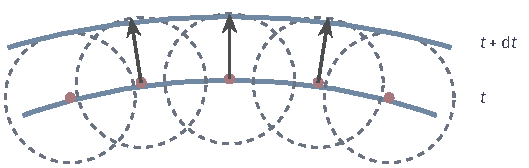
\includegraphics[width=89.5mm]{figures/06-differential-equations/02-partial-differential-equations/tikz/hj-huygens/figure.pdf}
  \caption{波前的包络图景。下方蓝线是时刻$t$的波前，红点发出半径$c\,\mathrm{d}t$的小圆（虚线），上方蓝线是这些小圆的包络，即$t+\mathrm{d}t$的波前，深灰箭头是射线。}
  \label{fig:hj-huygens}
\end{BookInlineFigure}

速度为常数时，$\nabla c=\bm{0}$，$\bm{p}$不变，射线是直线，$T$就是到源点的距离除以$c$。速度随位置变化时射线弯曲。例如在平面上取$c(\bm{x})=1+ax_2$，$a=1/2$，源在原点。这个速度下到达时间有闭式
\begin{equation}
  T(\bm{x})=\frac{1}{a}\operatorname{arccosh}\Bigl(1+\frac{a^2\lVert\bm{x}\rVert_2^2}{2c(\bm{x})}\Bigr),
  \label{eq:hj-linear-speed}
\end{equation}
代入程函方程可以验证。我们沿竖直射线手算一个点：在$x_1=0$上向上走，$\dot{x}_2=1+x_2/2$，$x_2(0)=0$，解得
\[
  x_2(t)=2\bigl(\mathrm{e}^{t/2}-1\bigr).
\]
令$x_2=2$，得到$t=2\ln2\approx1.386$。式~\eqref{eq:hj-linear-speed}在$(0,2)$处给出$\operatorname{arccosh}(1.25)/a=2\ln2$，两者一致。

图~\ref{fig:hj-rays-linear-speed}用数值积分解特征方程组，得到射线，再画上式~\eqref{eq:hj-linear-speed}的等值线。射线总向速度小的一侧弯转，斜向上出发的射线进入快层后又折回下方。射线与等值线处处垂直。积分到$t=3.2$时，射线终点的$T$值与$t$的差不超过$2\times10^{-11}$。

\begin{BookInlineFigure}
  \centering
  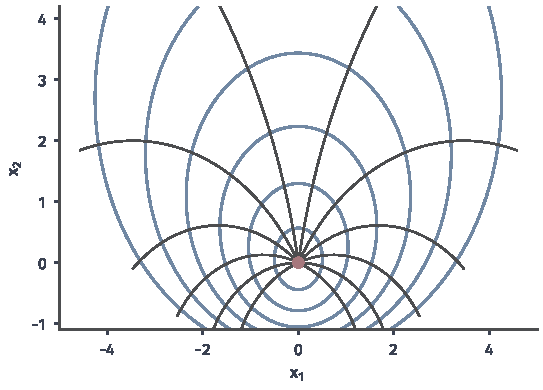
\includegraphics[width=92mm]{figures/06-differential-equations/02-partial-differential-equations/matplotlib/hj-rays-linear-speed/figure.pdf}
  \caption{速度$c=1+x_2/2$下从原点（红）出发的波前和射线。蓝线是式~\eqref{eq:hj-linear-speed}在$T=0.5,1,\ldots,3$的等值线，深灰线是用步长$0.01$的四阶Runge--Kutta方法积分特征方程组得到的射线，初始方向间隔$20^\circ$。}
  \label{fig:hj-rays-linear-speed}
\end{BookInlineFigure}

\paragraph{边界数据怎样启动特征线}
初值问题的特征线从每个$\bm{y}$以确定的斜率出发。程函方程的数据只在$\Gamma$上给出值，切向导数能由$g$算出，法向导数却要由方程决定。设$\Gamma$是一段超曲面，$\nabla_\Gamma g$是$g$沿$\Gamma$的切向梯度，$\bm{n}$是单位法向。令$\bm{p}=\nabla_\Gamma g+\beta\bm{n}$，代入$\lVert\bm{p}\rVert_2=1/c$，得到
\begin{equation}
  \beta=\pm\sqrt{\frac{1}{c^2}-\lVert\nabla_\Gamma g\rVert_2^2}.
  \label{eq:hj-boundary-branches}
\end{equation}
图~\ref{fig:hj-boundary-branches}的圆是$\lVert\bm{p}\rVert_2=1/c$，竖直虚线是切向分量固定时的所有候选，两个交点就是式~\eqref{eq:hj-boundary-branches}的两支。

\begin{BookInlineFigure}
  \centering
  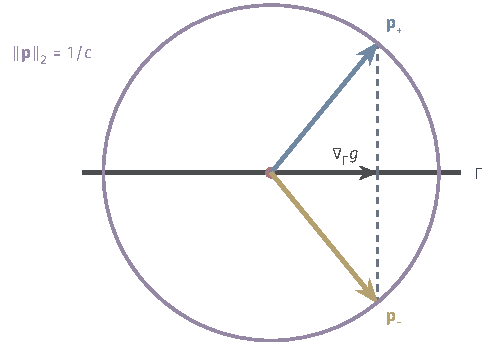
\includegraphics[width=83.5mm]{figures/06-differential-equations/02-partial-differential-equations/tikz/hj-boundary-branches/figure.pdf}
  \caption{边界上的初始斜率。紫圆是$\lVert\bm{p}\rVert_2=1/c$，水平线是边界$\Gamma$，切向分量$\nabla_\Gamma g$由数据给定，方程留下两支法向分量：$\bm{p}_+$（蓝）指向一侧，$\bm{p}_-$（黄）指向另一侧。}
  \label{fig:hj-boundary-branches}
\end{BookInlineFigure}

要使两支是不同的实数，需要$\lVert\nabla_\Gamma g\rVert_2<1/c$。它的含义是：起始时刻沿$\Gamma$变化得不能太快。沿$\Gamma$的视在传播速度$1/\lVert\nabla_\Gamma g\rVert_2$要大于当地的波速$c$。若$g$沿$\Gamma$变化得更快，某个点规定的起始时刻已晚于别的点传来的波前，就是第~\ref{sec:hj-problem}节$g(1)=2$的情形。选定一支后，就得到从$\Gamma$的一侧发出的波前。

\section{尖点的产生}
\label{sec:hj-cusps}

定理~\ref{thm:hj-local-classical}只保证短时间内有解。时间一长，映射$\bm{y}\mapsto\bm{x}(\bm{y},t)$可能不再可逆，同一个位置会被几条特征线到达。这时经典解到了尽头，而且仅仅要求方程几乎处处成立，也无法决定接下来该怎么办。

\paragraph{梯度沿特征线的变化}
取$d=1$，$H=H(p)$。此时$\dot{p}=-\partial_xH=0$，斜率沿特征线不变，特征线是直线：
\[
  x(y,t)=y+tH'\bigl(u_0'(y)\bigr).
\]
对$y$求导，记$a(y)=H''(u_0'(y))\,u_0''(y)$，得到
\[
  \partial_yx=1+ta(y).
\]

二阶导数$w=\partial_x^2u$沿特征线的取值，可以用$\partial_yp/\partial_yx$算出。由$p=u_0'(y)$，
\begin{equation}
  w(y,t)=\frac{u_0''(y)}{1+ta(y)}.
  \label{eq:hj-riccati}
\end{equation}
若$H$是严格凸的，$a(y)<0$恰好发生在$u_0''(y)<0$的地方，也就是初值向下弯的地方。这些地方的分母随时间减小，到$t=-1/a(y)$时变成零，曲率发散。

\begin{theorem}[经典解的首次失效]
\label{thm:hj-breakdown}
设$d=1$，$H\in C^2$，$u_0\in C^2$，且$u_0'$、$u_0''$有界，$H''$在$u_0'$的值域上有界。记$m=\inf_ya(y)$。

若$m\geq0$，令$t^*=\infty$；若$m<0$，令$t^*=-1/m$。则在$0\leq t<t^*$上，$y\mapsto x(y,t)$是$\mathbb{R}$到$\mathbb{R}$的同胚，特征线给出整个$\mathbb{R}\times[0,t^*)$上的$C^2$解。若$m<0$且下确界在某点$y^*$处达到，则
\begin{equation}
  \lim_{t\uparrow t^*}\bigl\lvert\partial_x^2u(x(y^*,t),t)\bigr\rvert=\infty,
  \label{eq:hj-breakdown}
\end{equation}
所以这个解不能在$t^*$之后作为$C^2$解延拓。
\end{theorem}

\begin{proof}
设$0\leq t<t^*$。此时
\[
  \partial_yx=1+ta(y)\geq1+tm\geq\kappa>0,
\]
其中$m\geq0$时取$\kappa=1$，$m<0$时取$\kappa=1-t/t^*$。一阶导数有正下界，所以$y\mapsto x$严格递增，并且$\lvert x\rvert\to\infty$（$\lvert y\rvert\to\infty$时），是同胚。

在每个闭区间$[0,t_2]\subset[0,t^*)$上，$\kappa$有统一的正下界。逐点应用定理~\ref{thm:hj-local-classical}的计算，得到连续可微的$u$，且$\partial_xu=p$。由$w$的公式，$\partial_xu$关于$x$连续可微，$u$是$C^2$解。

式~\eqref{eq:hj-breakdown}由式~\eqref{eq:hj-riccati}得到：在$y=y^*$处，分母是$1+tm=1-t/t^*\to0$，分子$u_0''(y^*)$不为零（因为$a(y^*)=m<0$）。若存在$C^2$延拓，$\partial_x^2u$在紧集上有界，这与发散矛盾。
\end{proof}

定理说的是：斜率的变化率在有限时间内发散，而斜率和场值本身一直有界。这和第~\ref{chap:scalar-conservation-laws}章的结论对应，$v=\partial_xu$正是在同一时刻由光滑变成间断。

把定理用到例~\ref{ex:hj-cos}。$a(y)=u_0''(y)=-\cos y$，最小值$-1$在$y=0$处取得，所以$t^*=1$。特征线和曲率是
\[
  \partial_yx=1-t\cos y,\qquad w=\frac{-\cos y}{1-t\cos y}.
\]
在$x=0$（$y=0$）处，$w=-1/(1-t)$。$t=0.5$时曲率是$-2$，$t=0.9$时是$-10$。图~\ref{fig:hj-cos-steepening}显示$u$在原点越来越尖，斜率曲线越来越陡。

\begin{BookInlineFigure}
  \centering
  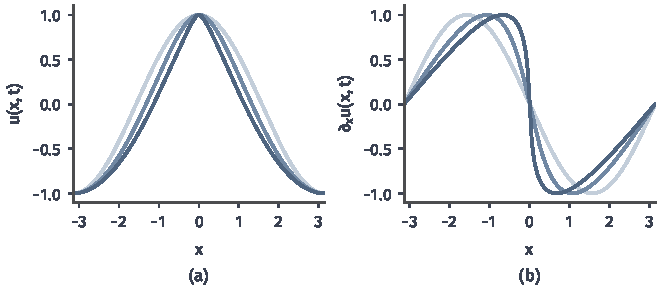
\includegraphics[width=112mm]{figures/06-differential-equations/02-partial-differential-equations/matplotlib/hj-cos-steepening/figure.pdf}
  \caption{$H=p^2/2$、$u_0=\cos x$的经典解，蓝色由浅到深是$t=0,0.5,0.9$。(a)场值$u$。(b)斜率$\partial_xu$，$x=0$处的斜率变化率是$-1/(1-t)$，$t\uparrow1$时发散，而斜率一直保持在$[-1,1]$内。}
  \label{fig:hj-cos-steepening}
\end{BookInlineFigure}

图~\ref{fig:hj-cos-characteristics}(a)把特征线全部画出来。$t<1$时它们互不相交，$t=1$时最先在红点相遇。条件$\partial_yx=0$给出特征线族的包络
\[
  t=\frac{1}{\cos y},\qquad x=y-\tan y,
\]
即图中的深灰曲线，称为\term{焦散线}（caustic）。两支焦散线之间的每个点都有三条特征线经过，这个区域由红点向上张开。

\begin{BookInlineFigure}
  \centering
  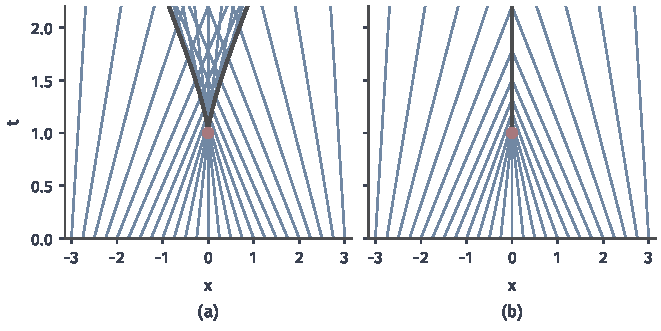
\includegraphics[width=112mm]{figures/06-differential-equations/02-partial-differential-equations/matplotlib/hj-cos-characteristics/figure.pdf}
  \caption{$u_0=\cos x$的特征线$x=y-t\sin y$（蓝）。(a)全部画出，它们在红点$(0,1)$首次相遇，深灰曲线是焦散线。(b)只画到撞上$x=0$（深灰粗线）为止的部分，第~\ref{sec:hj-hopf-lax}节将说明解用到的正是这一部分。}
  \label{fig:hj-cos-characteristics}
\end{BookInlineFigure}

\paragraph{同一位置的多个分支}
$t^*$之后，公式仍然能算，只是不再给出函数。取$t=\pi/2$、$x=0$，要求解
\[
  y=\frac{\pi}{2}\sin y.
\]
它有三个解$y=0$、$y=\pi/2$、$y=-\pi/2$。代入$p=-\sin y$和$z=\cos y+\frac{t}{2}\sin^2y$，得到
\[
  \begin{gathered}
    y=0:\quad(p,z)=(0,1),\\
    y=\tfrac{\pi}{2}:\quad(p,z)=(-1,\tfrac{\pi}{4}),\\
    y=-\tfrac{\pi}{2}:\quad(p,z)=(1,\tfrac{\pi}{4}).
  \end{gathered}
\]
三条特征线带来三对不同的斜率和值，$u(0,\pi/2)$应当取哪一个？特征方程组只负责沿线传递，回答不了这个问题。

图~\ref{fig:hj-swallowtail}(a)是$t=\pi/2$时$(x,z)$的像。曲线在$\lvert x\rvert\leq0.33$内折叠成三层，整条曲线不是函数图像。图(b)是相平面上$(x,p)$的像，初始的正弦曲线被Hamilton流剪切后折叠，同一个$x$上有三个$p$。蓝色画的是后面选出的解，下包络在$x=0$处有折角，斜率从$+1$跳到$-1$。

\begin{BookInlineFigure}
  \centering
  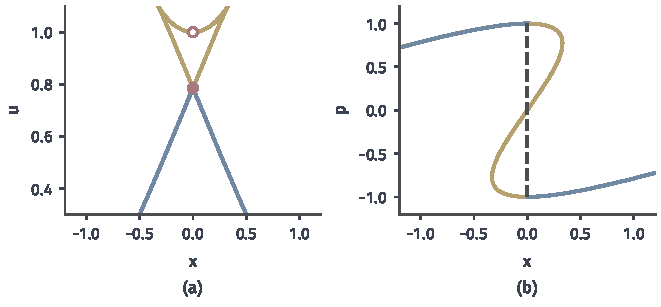
\includegraphics[width=112mm]{figures/06-differential-equations/02-partial-differential-equations/matplotlib/hj-swallowtail/figure.pdf}
  \caption{$t=\pi/2$时的多值像（黄）与选出的解（蓝）。(a)$(x,z)$平面，$x=0$处有三个值，红点是$\pi/4$（两条分支的公共值），空心点是$1$。(b)$(x,p)$平面，折叠的曲线在$x=0$处被虚线截断，蓝线在$x=0$处从$p=1$跳到$p=-1$。}
  \label{fig:hj-swallowtail}
\end{BookInlineFigure}

到达时间问题里，这个选择有明确的物理含义。平面上有两个源$\bm{a}=(-1,0)$和$\bm{b}=(1,0)$，时刻$0$同时点燃。每个源单独产生的到达时间是$T_1=\lVert\bm{x}-\bm{a}\rVert_2$和$T_2=\lVert\bm{x}-\bm{b}\rVert_2$，都是经典解。但一点只会被第一次到达的波前扫到，所以
\[
  T=\min\{T_1,T_2\}.
\]
后到的波前经过的是已经扫过的区域，没有意义。

图~\ref{fig:hj-two-sources}(a)显示两列圆形波前相遇后在中垂线上消失，$T$沿这条线不可微。在直线$x_2=1$上看，两条分支在$x_1=0$处都等于$\sqrt2$，斜率分别是$+1/\sqrt2$和$-1/\sqrt2$，取最小值后在该点形成折角，见图(b)。

\begin{BookInlineFigure}
  \centering
  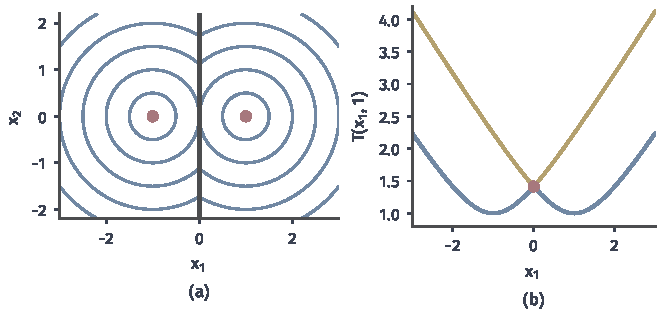
\includegraphics[width=112mm]{figures/06-differential-equations/02-partial-differential-equations/matplotlib/hj-two-sources/figure.pdf}
  \caption{两个同时点燃的源（红点）。(a)蓝线是$T=\min\{T_1,T_2\}$的等值线，深灰线是中垂线，两列波前在此相遇后消失。(b)沿$x_2=1$的截面，黄线是两个单独的到达时间，蓝线是取最小值的结果，红点是折角，高度$\sqrt2$。}
  \label{fig:hj-two-sources}
\end{BookInlineFigure}

这两个例子都选了较小的值。这究竟是巧合，还是方程本身的要求？下面的例子说明，光凭几乎处处的逐点检验回答不了。

\paragraph{几乎处处满足方程仍然不够}
取$H=p^2/2$，$u_0=0$。$u\equiv0$满足方程和初值。还有没有别的连续解？令
\begin{equation}
  w(x,t)=\min\Bigl\{\lvert x\rvert-\frac{t}{2},\ 0\Bigr\}.
  \label{eq:hj-notch}
\end{equation}
它的形状是一个越挖越深的凹槽，在$\lvert x\rvert\geq t/2$上等于$0$，在$\lvert x\rvert<t/2$上等于$\lvert x\rvert-t/2$。

逐块验证。在$\lvert x\rvert>t/2$上$w=0$，方程成立。在$0<\lvert x\rvert<t/2$上$\partial_xw=\pm1$，$\partial_tw=-1/2$，所以
\[
  \partial_tw+\frac12(\partial_xw)^2=-\frac12+\frac12=0.
\]
除了三条线$x=0$、$x=\pm t/2$，方程都成立，这三条线的测度为零。初值也满足。于是$w$和$0$是同一个初值问题的两个几乎处处解，见图~\ref{fig:hj-notch}(a)。

图~\ref{fig:hj-notch}(b)把凹槽翻译成斜率。$v=\partial_xw$在$x=\pm t/2$处的跳跃满足Rankine--Hugoniot条件，例如$x=t/2$处左值$1$、右值$0$，通量$v^2/2$给出速度$1/2$。而在$x=0$处，$v$从$-1$跳到$+1$，这是左值小于右值的间断。第~\ref{chap:scalar-conservation-laws}章的熵条件说，凸通量下的间断必须左值大于右值，否则特征线会从间断面向外分开。$x=0$处的跳跃正好违反这一条。

\begin{BookInlineFigure}
  \centering
  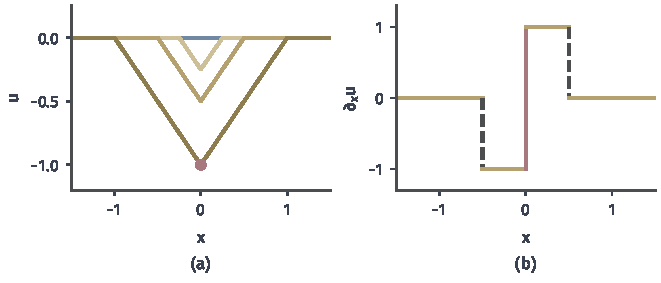
\includegraphics[width=112mm]{figures/06-differential-equations/02-partial-differential-equations/matplotlib/hj-notch/figure.pdf}
  \caption{初值为$0$时的非唯一性。(a)蓝线是$u=0$，黄色由浅到深是式~\eqref{eq:hj-notch}的$w$在$t=0.5,1,2$的图像，红点是底部折角。(b)$t=1$时的斜率$\partial_xw$，深灰虚线处的跳跃左值大于右值，红线处的跳跃左值小于右值。}
  \label{fig:hj-notch}
\end{BookInlineFigure}

因此，光用“几乎处处”这条标准，经典解失效后方程给不出答案。需要在不可微的点上也提出要求，而且要求必须能区分$w$底部的折角和$T$的尖峰。这是下一节的任务。

\section{黏性解}
\label{sec:hj-viscosity}

折角处没有导数，方程不能代入。能否用一些有导数的东西替代它？答案是拿光滑函数从上方或下方贴住$u$，把方程写在贴住的光滑函数上。

\paragraph{用光滑函数从两侧接触}
设$\varphi$是光滑函数，$u-\varphi$在点$\bm{x}_0$有局部极大值。几何上，把$\varphi$上下平移，使它在$\bm{x}_0$处与$u$相等，那么附近有$\varphi\geq u$，$\varphi$从上方贴住$u$。若$u$在$\bm{x}_0$可微，极值点的一阶条件给出$\nabla\varphi(\bm{x}_0)=\nabla u(\bm{x}_0)$。这样可以从$\varphi$读出$u$的梯度。

$u$不可微时，情况由折角的方向决定。图~\ref{fig:hj-touching}画了三种情形。在光滑点上，从上方和下方都能贴住，贴住的函数斜率都等于$u$的斜率。在向下弯的折角（凹折角）处，从上方可以用多种斜率贴住，从下方则根本贴不住。在向上弯的折角（凸折角）处正好相反。

\begin{BookInlineFigure}
  \centering
  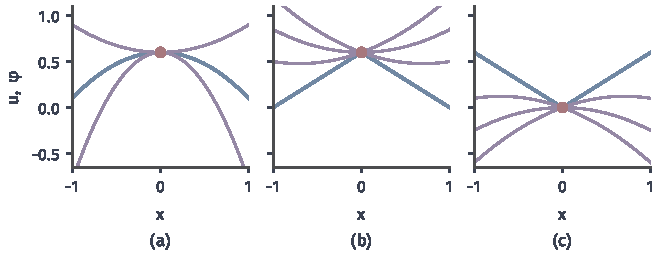
\includegraphics[width=112mm]{figures/06-differential-equations/02-partial-differential-equations/matplotlib/hj-touching/figure.pdf}
  \caption{光滑测试函数（紫）在红点贴住$u$（蓝）。(a)光滑点：上下两侧都能贴住，斜率唯一。(b)凹折角：只能从上方贴住，斜率可取一个区间。(c)凸折角：只能从下方贴住，斜率可取一个区间。}
  \label{fig:hj-touching}
\end{BookInlineFigure}

接下来决定不等式的方向。设$u_\varepsilon$是$\partial_tu+H(\nabla u)=\varepsilon\Delta u$的光滑解，$\varepsilon>0$，且$u_\varepsilon-\varphi$在内部点取局部极大。一阶条件和二阶条件给出
\[
  \partial_t\varphi=\partial_tu_\varepsilon,\qquad\nabla\varphi=\nabla u_\varepsilon,\qquad\Delta u_\varepsilon\leq\Delta\varphi.
\]
代入方程，得到
\[
  \partial_t\varphi+H(\nabla\varphi)=\varepsilon\Delta u_\varepsilon\leq\varepsilon\Delta\varphi.
\]
令$\varepsilon\to0$，右端趋于零。所以从上方贴时，自然的要求是$\partial_t\varphi+H(\nabla\varphi)\leq0$；从下方贴时不等号反向。这个计算只是启示，严格的结论在第~\ref{sec:hj-vanishing}节证明，但它已经给出了定义的形状。

\begin{definition}[黏性解]
\label{def:hj-viscosity}
设$u\in C(\mathbb{R}^{d}\times[0,t_{\mathrm{f}}))$。若对每个$\varphi\in C^1(\mathbb{R}^{d}\times(0,t_{\mathrm{f}}))$，当$u-\varphi$在$(\bm{x}_0,t_0)$（$t_0>0$）取局部极大值时都有
\begin{equation}
  \partial_t\varphi(\bm{x}_0,t_0)+H\bigl(t_0,\bm{x}_0,\nabla\varphi(\bm{x}_0,t_0)\bigr)\leq0,
  \label{eq:hj-subsolution}
\end{equation}
就称$u$是式~\eqref{eq:hj-ivp}中方程的\term{黏性次解}（viscosity subsolution）。若对每个这样的$\varphi$，当$u-\varphi$在$(\bm{x}_0,t_0)$取局部极小值时都有
\begin{equation}
  \partial_t\varphi(\bm{x}_0,t_0)+H\bigl(t_0,\bm{x}_0,\nabla\varphi(\bm{x}_0,t_0)\bigr)\geq0,
  \label{eq:hj-supersolution}
\end{equation}
就称$u$是\term{黏性上解}（viscosity supersolution）。既是次解又是上解的函数称为黏性解。初值问题的黏性解还要求$u(\cdot,0)=u_0$。
\end{definition}

记忆方式是：次解贴上方，得到“小于等于”；上解贴下方，得到“大于等于”。这个定义里从头到尾没有$u$的导数，所以它对连续函数有意义。

稳态方程$F(\bm{x},\nabla u)=0$的定义完全相同：局部极大处要求$F(\bm{x}_0,\nabla\varphi)\leq0$，局部极小处要求$F(\bm{x}_0,\nabla\varphi)\geq0$，边界条件单独提出。到达时间问题取
\[
  F(\bm{x},\bm{p})=c(\bm{x})\lVert\bm{p}\rVert_2-1.
\]

定义要有用，首先不能把经典解排除在外，而且不可微的地方之外应当和原方程一致。

\begin{lemma}[与经典解相容]
\label{lem:hj-consistency}
(1)连续可微的经典解是黏性解。(2)若黏性解$u$在内部点$\bm{z}_0=(\bm{x}_0,t_0)$可微，则方程在$\bm{z}_0$处逐点成立，即
\begin{equation}
  \partial_tu(\bm{z}_0)+H\bigl(t_0,\bm{x}_0,\nabla u(\bm{z}_0)\bigr)=0.
  \label{eq:hj-consistency}
\end{equation}
\end{lemma}

\begin{proof}
(1)若$u\in C^1$，$u-\varphi$在内部取极值，则$\partial_t\varphi=\partial_tu$，$\nabla\varphi=\nabla u$，代入方程得到等号，两个不等式都成立。

(2)只需构造一个$C^1$函数从上方贴住$u$且导数与$u$相同，下方同理，再分别代入两个定义。记$r=\lVert\bm{z}-\bm{z}_0\rVert_2$，并令$v$为$u$减去它在$\bm{z}_0$的一阶Taylor多项式。由可微性，
\[
  \rho(r)=\max_{\lVert\bm{z}-\bm{z}_0\rVert_2\leq r}\frac{\lvert v(\bm{z})\rvert}{\lVert\bm{z}-\bm{z}_0\rVert_2}
\]
连续、不减，且$\rho(0)=0$（规定分式在$\bm{z}=\bm{z}_0$处取$0$）。令
\[
  \psi(\bm{z})=\int_r^{2r}\rho(\tau)\,\mathrm{d}\tau.
\]

$\rho$连续，所以$\psi$在$\bm{z}\neq\bm{z}_0$处$C^1$。又$\lvert\psi\rvert\leq r\rho(2r)=o(r)$，所以$\psi$在$\bm{z}_0$处可微且导数为零，导数的表达式也趋于零，$\psi\in C^1$。由$\rho$不减，得$\psi(\bm{z})\geq r\rho(r)\geq v(\bm{z})$。

于是$v-\psi$在$\bm{z}_0$有局部极大值$0$，以“一阶Taylor多项式$+\psi$”作测试函数代入式~\eqref{eq:hj-subsolution}，得到式~\eqref{eq:hj-consistency}左端$\leq0$。用$-\psi$代替$\psi$，由式~\eqref{eq:hj-supersolution}得到$\geq0$。
\end{proof}

Lipschitz函数几乎处处可微（Rademacher定理，证明要用到Lebesgue微分定理和逐方向的论证，篇幅较长，读者可查阅实分析教材），所以Lipschitz连续的黏性解几乎处处满足方程。黏性解比“几乎处处解”多出来的，是在余下的零测集上的不等式。

下面的引理很快会用到：Lipschitz函数被贴住时，测试函数的斜率不会超过Lipschitz常数。

\begin{lemma}[贴住Lipschitz函数]
\label{lem:hj-lipschitz-touch}
设$u$关于$\bm{x}$是$R$-Lipschitz的，$\varphi\in C^1$，$u-\varphi$在$(\bm{x}_0,t_0)$取局部极大值或局部极小值，则
\begin{equation}
  \lVert\nabla\varphi(\bm{x}_0,t_0)\rVert_2\leq R.
  \label{eq:hj-lipschitz-touch}
\end{equation}
\end{lemma}

\begin{proof}
设取局部极大值，$t$固定为$t_0$。对单位向量$\bm{e}$和小$h>0$，有
\[
  \varphi(\bm{x}_0+h\bm{e},t_0)-\varphi(\bm{x}_0,t_0)\geq u(\bm{x}_0+h\bm{e},t_0)-u(\bm{x}_0,t_0)\geq-Rh.
\]
除以$h$并令$h\to0$，得到$\langle\nabla\varphi,\bm{e}\rangle\geq-R$。取$\bm{e}=-\nabla\varphi/\lVert\nabla\varphi\rVert_2$，就得到结论。局部极小的情形把$u-\varphi$换成$\varphi-u$。
\end{proof}

\paragraph{折角检验}
回到程函方程$\lvert u'\rvert=1$，$u(\pm1)=0$，这里$F(p)=\lvert p\rvert-1$。检验两个候选。

\begin{example}[两个折角]
\label{ex:hj-kink-test}
候选一$u=1-\lvert x\rvert$。在$x\neq0$处它光滑且满足方程，只需检验$x=0$。从下方贴不住（$x=0$是凹折角），所以上解条件是空的。从上方贴住时，$\varphi'(0)=p$满足$\lvert p\rvert\leq1$，于是
\[
  F(p)=\lvert p\rvert-1\leq0.
\]
次解条件成立，$1-\lvert x\rvert$是黏性解。

候选二$u=\lvert x\rvert-1$。$x=0$是凸折角，从上方贴不住，从下方能贴住。取$\varphi\equiv-1$，它从下方贴住$u$，斜率为$0$。上解条件要求
\[
  F(0)=-1\geq0,
\]
这不成立，所以$\lvert x\rvert-1$不是黏性解。
\end{example}

图~\ref{fig:hj-kink-test}展示了这两个检验。第~\ref{chap:pde-problems}章的每条锯齿线都有凸折角，同样在那里失败。凹折角和凸折角的差别就是答案：凸折角要求贴住的斜率长度至少为$1$，而$[-1,1]$内的斜率都能贴住，这不可能；凹折角要求长度至多为$1$，恰好成立。

\begin{BookInlineFigure}
  \centering
  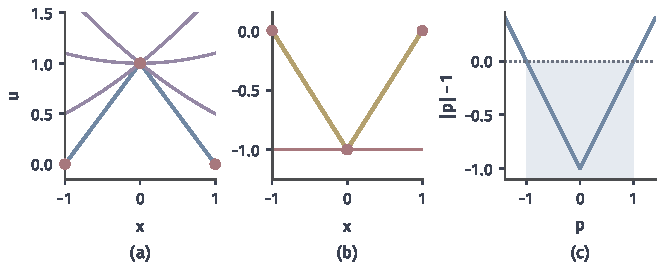
\includegraphics[width=112mm]{figures/06-differential-equations/02-partial-differential-equations/matplotlib/hj-kink-test/figure.pdf}
  \caption{程函方程$\lvert u'\rvert=1$（红点为边值）的折角检验。(a)$1-\lvert x\rvert$在顶点被紫线从上方贴住，斜率在$[-1,1]$内。(b)$\lvert x\rvert-1$在底点被水平红线从下方贴住，斜率$0$。(c)$\lvert p\rvert-1$，浅蓝范围内它不大于$0$：次解条件成立而上解条件不成立。}
  \label{fig:hj-kink-test}
\end{BookInlineFigure}

这个检验在到达时间问题中有直观的含义。若$T$在内部有凸折角，那么该点比它左右两边都早被到达，可是波前只能从相邻位置传来，内部没有源的地方不可能出现这种情况。凹折角则是两列波前相遇的地方，这是允许的。

定义对方程的符号敏感。把$F$换成$-F$，上下解的角色互换，方程$-\lvert u'\rvert+1=0$的黏性解是$\lvert x\rvert-1$，而不是$1-\lvert x\rvert$。这一点和弱解不同：弱形式乘$-1$不改变解集。这里的符号规定了信息传播的方向，$\partial_tu+H=0$中$\partial_tu$的系数为正，这是时间向前的方向。

对高维的到达时间问题，同样的两步检验可以直接做。

\begin{theorem}[距离函数]
\label{thm:hj-distance}
设$\Omega\subset\mathbb{R}^{d}$是开集，$\Omega\neq\mathbb{R}^{d}$，$u(\bm{x})$是$\bm{x}$到$\partial\Omega$的最短欧氏距离。则$u$是
\begin{equation}
  \lVert\nabla u\rVert_2-1=0\quad\text{在}\ \Omega\ \text{内}
  \label{eq:hj-distance}
\end{equation}
的黏性解。
\end{theorem}

\begin{proof}
三角不等式说明$u$是$1$-Lipschitz的。局部极大处，由引理~\ref{lem:hj-lipschitz-touch}得$\lVert\nabla\varphi\rVert_2\leq1$，次解条件成立。

设$u-\varphi$在$\bm{x}\in\Omega$取局部极小值，$\bm{y}\in\partial\Omega$是最近点，$\bm{e}$是从$\bm{x}$指向$\bm{y}$的单位向量。对小$h>0$，$\bm{x}_h=\bm{x}+h\bm{e}$仍在$\Omega$内，并且
\[
  u(\bm{x}_h)\leq\lVert\bm{x}_h-\bm{y}\rVert_2=u(\bm{x})-h.
\]
由局部极小，得到
\[
  \varphi(\bm{x}_h)-\varphi(\bm{x})\leq u(\bm{x}_h)-u(\bm{x})\leq-h.
\]
除以$h$并令$h\to0$，得到$\langle\nabla\varphi,\bm{e}\rangle\leq-1$，所以$\lVert\nabla\varphi(\bm{x})\rVert_2\geq1$，上解条件成立。
\end{proof}

取$\Omega=\mathbb{R}^2\setminus\{\bm{a},\bm{b}\}$，就知道图~\ref{fig:hj-two-sources}的$T=\min\{T_1,T_2\}$是黏性解。“第一次到达”这个物理选择，在方程层面就是黏性条件。

\paragraph{时间依赖的折角}
再回到凹槽$w$。它在$(0,t)$处的折角和$(t/2,t)$处的折角方向相反，检验结果也相反。

\begin{example}[凹槽不是黏性解]
\label{ex:hj-notch-test}
在$t_0>0$的点$(0,t_0)$附近，$w=\lvert x\rvert-t/2$。函数$\varphi=-t/2$从下方贴住$w$，其$q=\partial_t\varphi=-1/2$，$p=\partial_x\varphi=0$。上解条件要求
\[
  q+\frac{p^2}{2}=-\frac12\geq0,
\]
不成立，所以$w$不是上解。

对比$x=t/2$的折角。在那里$w=\min\{x-t/2,\ 0\}$，从上方贴住的测试函数，其$(q,p)$落在两个平面梯度$(-\tfrac12,1)$和$(0,0)$的连线上，写成$(q,p)=(-s/2,s)$，$0\leq s\leq1$。代入得到
\[
  q+\frac{p^2}{2}=-\frac{s}{2}+\frac{s^2}{2}\leq0,
\]
次解条件成立。这个折角是允许的。
\end{example}

图~\ref{fig:hj-notch-test}是这两个量。第一个折角对应$v$的左值小于右值的跳跃，第二个对应左值大于右值的跳跃，这和第~\ref{sec:hj-cusps}节由熵条件得到的判断一致。黏性解的定义不用导数，却自动区分了这两种跳跃。

\begin{BookInlineFigure}
  \centering
  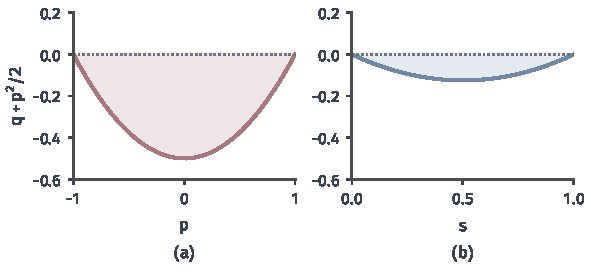
\includegraphics[width=100mm]{figures/06-differential-equations/02-partial-differential-equations/matplotlib/hj-notch-test/figure.pdf}
  \caption{凹槽$w$两类折角上的检验量$q+p^2/2$。(a)底部$x=0$处，$q=-1/2$，$\lvert p\rvert\leq1$，红线全部为负，上解条件不满足。(b)$x=t/2$处，$(q,p)=(-s/2,s)$，蓝线全部非正，次解条件满足。}
  \label{fig:hj-notch-test}
\end{BookInlineFigure}

\paragraph{与弱解的区别}
黏性解和弱解都用测试函数，但做的事情不一样。弱解把方程乘上测试函数积分，导数通过分部积分转到测试函数上，方程必须有散度形式。黏性解不做积分，也不移走导数，它只在测试函数贴住解的一点上读取一阶导数，建立一个微分不等式。表~\ref{tab:hj-weak-vs-viscosity}把两者并列。

\begin{BookInlineTable}
  \centering
  \begin{tabular}{lll}
    \toprule
    & 弱解 & 黏性解\\
    \midrule
    测试函数的角色 & 乘上去做积分 & 在接触点处提供导数\\
    检验位置 & 整个区域的积分 & 逐点的不等式\\
    需要的结构 & 散度形式 & 方程的符号（单调性）\\
    方程乘$-1$ & 解不变 & 解改变\\
    对极限的稳定性 & 弱收敛下通量要可控 & 局部一致收敛即可\\
    \bottomrule
  \end{tabular}
  \caption{弱解与黏性解的对比。}
  \label{tab:hj-weak-vs-viscosity}
\end{BookInlineTable}

所以黏性解并不是把方程积分一下得到的弱化形式，$H(\nabla u)$非线性时，分部积分本来就做不了。这个定义的价值要由下一节的比较原理来兑现。

\section{比较原理}
\label{sec:hj-comparison}

黏性解的定义只是几条不等式，它能确定唯一的函数吗？在到达时间的语言里，答案应当由一个朴素的事实决定：更早点燃的波前不会更晚到达。把它写成数学就是比较原理：次解在初始或边界上不超过上解，就处处不超过上解。

\paragraph{光滑情形的机制}
先看$u$、$v$都光滑的情形，$u$是次解，$v$是上解，$u(\cdot,0)\leq v(\cdot,0)$。假设$u-v$在某处为正，为了简单，设最大值在$t_0>0$的某点$(\bm{x}_0,t_0)$取到。在这一点
\[
  \nabla u=\nabla v,\qquad\partial_tu\geq\partial_tv,
\]
后一个不等号是因为最大值的时刻可能是右端点。两个方程相减，两个$H$在同一个梯度上取值，相互抵消，得到$\partial_tu-\partial_tv\leq0$。

这还不是矛盾，$\partial_tu=\partial_tv$是可能的。修补的办法是减去一个严格增长的时间函数，例如$\lambda t$或$\lambda/(t_{\mathrm{f}}-t)$，使极大点处的时间导数严格大于零，这样就矛盾了。

对只连续的$u$、$v$，上面的第一式无法写出：在$u-v$的极大点，$u$和$v$都可能不可微。解决办法是\term{变量倍增}（doubling of variables）：用两组独立的变量分别处理$u$和$v$，并加上惩罚项迫使它们靠近，
\[
  \Phi(\bm{x},\bm{y})=u(\bm{x})-v(\bm{y})-\frac{\lVert\bm{x}-\bm{y}\rVert_2^2}{\delta^2}.
\]

固定$\bm{y}$时，$\Phi$是$u$减去一个光滑函数，这个光滑函数可以作为$u$的测试函数；固定$\bm{x}$时同样能作为$v$的测试函数。两个测试函数的梯度都是$2(\bm{x}-\bm{y})/\delta^2$，同一个$\bm{p}$出现在两边，这正是光滑情形下$\nabla u=\nabla v$的替身。

图~\ref{fig:hj-doubling}用一对带折角的函数演示。$\delta$变小时，$\Phi$的正值区域被压向对角线，极大点（绿）也靠向对角线，且其高度趋向$u-v$的最大值。

\begin{BookInlineFigure}
  \centering
  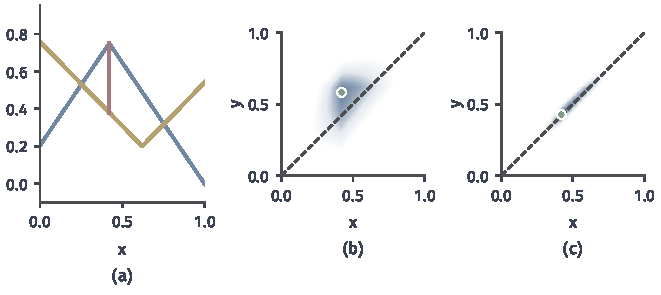
\includegraphics[width=112mm]{figures/06-differential-equations/02-partial-differential-equations/matplotlib/hj-doubling/figure.pdf}
  \caption{变量倍增。(a)$u$（蓝，凹折角）和$v$（黄，凸折角），红线段标出$u-v$的最大值。(b)、(c)$\Phi(x,y)$的正值，白色表示$\Phi\leq0$，蓝色越深值越大，绿点是极大点，虚线是对角线，$\delta=0.6$和$0.12$。}
  \label{fig:hj-doubling}
\end{BookInlineFigure}

\paragraph{初值问题}
下面是初值问题的比较原理。为了涵盖$H=p^2/2$这种关于$\bm{p}$不全局Lipschitz的情形，我们要求函数关于$\bm{x}$是Lipschitz的，这样只需要$H$在有界的$\bm{p}$上的性质。

\begin{theorem}[初值问题的比较原理]
\label{thm:hj-comparison}
设$H(t,\bm{x},\bm{p})$在$\lVert\bm{p}\rVert_2\leq R$的范围内关于全部自变量一致连续。设$u,v$在$\mathbb{R}^{d}\times[0,t_{\mathrm{f}}]$上有界、一致连续，关于$\bm{x}$是$R$-Lipschitz的，$u$是次解，$v$是上解。若$u(\cdot,0)\leq v(\cdot,0)$，则
\begin{equation}
  u\leq v\quad\text{在}\ \mathbb{R}^{d}\times[0,t_{\mathrm{f}}]\ \text{上}.
  \label{eq:hj-comparison}
\end{equation}
\end{theorem}

\begin{proof}
反设$\sigma=\sup(u-v)>0$。由连续性，存在$(\bar{\bm{x}},\bar{t})$，$\bar{t}<t_{\mathrm{f}}$，使$(u-v)(\bar{\bm{x}},\bar{t})>3\sigma/4$。对$\lambda,\delta>0$，记$\psi(t)=\lambda/(t_{\mathrm{f}}-t)$，并令
\[
  \begin{aligned}
    \Phi(\bm{x},\bm{y},t,s)={}&u(\bm{x},t)-v(\bm{y},s)-\psi(t)-\psi(s)\\
    &-\frac{\lVert\bm{x}-\bm{y}\rVert_2^2+(t-s)^2}{\delta^2}-\delta\bigl(\lVert\bm{x}\rVert_2^2+\lVert\bm{y}\rVert_2^2\bigr).
  \end{aligned}
\]
$\psi$在$t\to t_{\mathrm{f}}$时趋于无穷，二次项在无穷远处趋于负无穷，而$u,v$有界，所以$\Phi$在某点$(\bm{x}_0,\bm{y}_0,t_0,s_0)$取到最大值，且$t_0,s_0<t_{\mathrm{f}}$。先取$\lambda$充分小，此后只令$\delta\to0$，使得
\[
  \Phi(\bm{x}_0,\bm{y}_0,t_0,s_0)\geq\Phi(\bar{\bm{x}},\bar{\bm{x}},\bar{t},\bar{t})\geq\frac{\sigma}{2}.
\]

第一步估计最大点。记$C_0=\sup\lvert u\rvert+\sup\lvert v\rvert$。由上式，各惩罚项之和不超过$u(\bm{x}_0,t_0)-v(\bm{y}_0,s_0)\leq C_0$，所以
\[
  \begin{gathered}
    \lVert\bm{x}_0-\bm{y}_0\rVert_2\leq\sqrt{C_0}\,\delta,\qquad\lvert t_0-s_0\rvert\leq\sqrt{C_0}\,\delta,\\
    \delta\lVert\bm{x}_0\rVert_2\leq\sqrt{C_0\delta},\qquad\delta\lVert\bm{y}_0\rVert_2\leq\sqrt{C_0\delta}.
  \end{gathered}
\]

第二步说明$t_0,s_0>0$。若$t_0=0$，由$u(\cdot,0)\leq v(\cdot,0)$，
\[
  \frac{\sigma}{2}\leq u(\bm{x}_0,0)-v(\bm{y}_0,s_0)\leq v(\bm{x}_0,0)-v(\bm{y}_0,s_0).
\]
$s_0=\lvert t_0-s_0\rvert$，右端在$\delta\to0$时由$v$的一致连续性趋于零，矛盾。若$s_0=0$，同样用$u$的一致连续性得到矛盾。

第三步使用次解和上解的定义。记$\bm{p}=2(\bm{x}_0-\bm{y}_0)/\delta^2$。固定$(\bm{y}_0,s_0)$，函数$(\bm{x},t)\mapsto\Phi$是$u$减去$C^1$函数，它在$(\bm{x}_0,t_0)$取极大。测试函数的时间导数是$\psi'(t_0)+2(t_0-s_0)/\delta^2$，梯度是$\bm{p}+2\delta\bm{x}_0$，所以由次解条件，
\[
  \psi'(t_0)+\frac{2(t_0-s_0)}{\delta^2}+H\bigl(t_0,\bm{x}_0,\bm{p}+2\delta\bm{x}_0\bigr)\leq0.
\]

固定$(\bm{x}_0,t_0)$，$v$减去相应的$C^1$函数在$(\bm{y}_0,s_0)$取极小，测试函数的时间导数是$-\psi'(s_0)+2(t_0-s_0)/\delta^2$，梯度是$\bm{p}-2\delta\bm{y}_0$。由上解条件，
\[
  -\psi'(s_0)+\frac{2(t_0-s_0)}{\delta^2}+H\bigl(s_0,\bm{y}_0,\bm{p}-2\delta\bm{y}_0\bigr)\geq0.
\]

两式相减，$2(t_0-s_0)/\delta^2$抵消，得到
\[
  \psi'(t_0)+\psi'(s_0)\leq H\bigl(s_0,\bm{y}_0,\bm{p}-2\delta\bm{y}_0\bigr)-H\bigl(t_0,\bm{x}_0,\bm{p}+2\delta\bm{x}_0\bigr).
\]
由引理~\ref{lem:hj-lipschitz-touch}，两个梯度的长度都不超过$R$，所以可以用$H$的一致连续性。两组自变量的距离由第一步趋于零，右端趋于零。

而左端不小于$2\lambda/t_{\mathrm{f}}^2$，是一个与$\delta$无关的正数，矛盾。
\end{proof}

证明中每个假设的作用都能指出来。有界性让$\delta\lVert\bm{x}\rVert_2^2$这一项能把最大点留在有限范围内，这是增长条件的来源。一致连续性让第二步能把最大点推离$t=0$。Lipschitz条件和$H$的一致连续性负责最后一步。$\psi$的引入提供了严格的正数。

比较原理立刻给出唯一性和连续依赖。

\begin{theorem}[唯一性与数据稳定性]
\label{thm:hj-uniqueness}
在定理~\ref{thm:hj-comparison}的条件下，设$u$、$v$是黏性解，初值分别为$u_0$、$v_0$，$H$不依赖场值。则对$0\leq t\leq t_{\mathrm{f}}$，
\begin{equation}
  \sup_{\bm{x}}\lvert u(\bm{x},t)-v(\bm{x},t)\rvert\leq\sup_{\bm{x}}\lvert u_0(\bm{x})-v_0(\bm{x})\rvert.
  \label{eq:hj-stability}
\end{equation}
特别地，在这一函数类中，同一初值的黏性解至多一个。
\end{theorem}

\begin{proof}
记$K=\sup\lvert u_0-v_0\rvert$。$H$不依赖场值，所以$v+K$仍是黏性解，因为加常数不改变测试函数的导数。此时$u_0\leq v_0+K$，由比较原理得$u\leq v+K$。交换$u$、$v$得到另一半。$K=0$时就是唯一性。
\end{proof}

式~\eqref{eq:hj-stability}说明，解到解的映射在上确界范数下不扩张。图~\ref{fig:hj-order-preserved}用第~\ref{sec:hj-hopf-lax}节的公式算了一个例子：初值的差在$[0,0.6]$内，此后$u\leq v$一直保持，差的最大值始终不超过$0.6$，差的最小值保持为$0$。

\begin{BookInlineFigure}
  \centering
  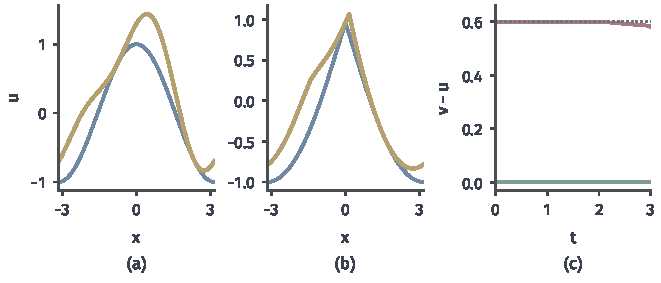
\includegraphics[width=112mm]{figures/06-differential-equations/02-partial-differential-equations/matplotlib/hj-order-preserved/figure.pdf}
  \caption{次序保持与上确界稳定性，$H=p^2/2$。(a)初值$u_0=\cos x$（蓝）和$v_0=\cos x+0.3+0.3\sin2x$（黄），$v_0\geq u_0$。(b)$t=1.2$的解，次序不变。(c)$v-u$的最大值（红）和最小值（绿）随时间的变化，虚线是初始最大差$0.6$。}
  \label{fig:hj-order-preserved}
\end{BookInlineFigure}

比较原理还给出简单的先验界。对$H=p^2/2$和例~\ref{ex:hj-cos}，常数$\pm1$都是经典解，$-1\leq\cos x\leq1$，所以在所有时刻$-1\leq u\leq1$。不解方程就知道了解的范围。

也可以用它解释凹槽为什么被排除。若$w$是上解，将它和次解$0$比较，初值都是$0$，比较原理给出$0\leq w$，而$w$在凹槽内为负。所以$w$不可能是上解，这就是例~\ref{ex:hj-notch-test}在底部折角处看到的失败。整体的比较结论，靠的正是接触点处的不等式。

条件不能随意去掉。取无界的初值$u_0=-x^2/2$，$H=p^2/2$，由特征线得到经典解
\[
  u(x,t)=-\frac{x^2}{2(1-t)},\qquad0\leq t<1.
\]
当$t\uparrow1$时，$u(x,t)\to-\infty$（$x\neq0$），没有办法延拓到$t\geq1$。有界性假设排除的就是这种从无穷远处传来的影响。

\paragraph{边值问题}
稳态的到达时间问题没有时间方向，上面证明中的$\psi$无从谈起，严格性要用别的办法得到。程函方程里可以把次解乘一个小于$1$的常数。

\begin{theorem}[程函方程的比较原理]
\label{thm:hj-comparison-eikonal}
设$\Omega\subset\mathbb{R}^{d}$有界开，$n\in C(\overline{\Omega})$，$n>0$。设$u,v\in C(\overline{\Omega})$分别是$\lVert\nabla u\rVert_2=n$在$\Omega$内的次解和上解，并且在$\partial\Omega$上$u\leq v$，则
\begin{equation}
  u\leq v\quad\text{在}\ \overline{\Omega}\ \text{上}.
  \label{eq:hj-comparison-eikonal}
\end{equation}
\end{theorem}

\begin{proof}
反设$\sigma=\max_{\overline{\Omega}}(u-v)>0$。取$\theta\in(0,1)$充分接近$1$，使$(1-\theta)\max\lvert u\rvert<\sigma/4$，于是$\sigma'=\max(\theta u-v)\geq3\sigma/4$，而在$\partial\Omega$上$\theta u-v\leq\sigma/4$。

对$\delta>0$，令
\[
  \Phi(\bm{x},\bm{y})=\theta u(\bm{x})-v(\bm{y})-\frac{\lVert\bm{x}-\bm{y}\rVert_2^2}{\delta^2},
\]
它在紧集$\overline{\Omega}\times\overline{\Omega}$上的最大点记为$(\bm{x}_\delta,\bm{y}_\delta)$。$\Phi$的最大值不小于$\sigma'$，所以惩罚项有界，$\lVert\bm{x}_\delta-\bm{y}_\delta\rVert_2\to0$。取子列使$\bm{x}_\delta,\bm{y}_\delta\to\bm{z}$，由连续性
\[
  \theta u(\bm{z})-v(\bm{z})\geq\sigma'\geq\frac{3\sigma}{4}.
\]
这说明$\bm{z}\notin\partial\Omega$，$\delta$小时$\bm{x}_\delta,\bm{y}_\delta$都在$\Omega$内。

记$\bm{p}=2(\bm{x}_\delta-\bm{y}_\delta)/\delta^2$。固定$\bm{y}_\delta$，$u$减去光滑函数在$\bm{x}_\delta$取极大，测试函数的梯度是$\bm{p}/\theta$，由次解条件$\lVert\bm{p}\rVert_2/\theta\leq n(\bm{x}_\delta)$。固定$\bm{x}_\delta$，由上解条件$\lVert\bm{p}\rVert_2\geq n(\bm{y}_\delta)$。两式合并，得到
\[
  n(\bm{y}_\delta)\leq\theta\,n(\bm{x}_\delta).
\]
令$\delta\to0$，$n(\bm{z})\leq\theta n(\bm{z})$，与$n(\bm{z})>0$、$\theta<1$矛盾。
\end{proof}

取$n=1/c$，$c$连续且有正的上下界，这个定理就适用于第~\ref{sec:hj-problem}节的到达时间问题，方程写成$c\lVert\nabla T\rVert_2-1=0$和$\lVert\nabla T\rVert_2-n=0$时次解、上解的条件相同，因为$c>0$不改变不等号方向。定理~\ref{thm:hj-distance}的距离函数在有界区域上是边值为零的唯一黏性解。

正性$n>0$的作用是提供严格性。若$n$在某点为零，可以看到比较原理失败。在$(-1,1)$上取$\lvert u'\rvert=2\lvert x\rvert$，$u(\pm1)=0$，这里$n(0)=0$，相当于速度在原点为无穷大。则
\[
  u=1-x^2\qquad\text{和}\qquad u=x^2-1
\]
都是$C^1$的经典解，因而都是黏性解，见图~\ref{fig:hj-boundary-failures}(a)。这就破坏了唯一性。

\begin{BookInlineFigure}
  \centering
  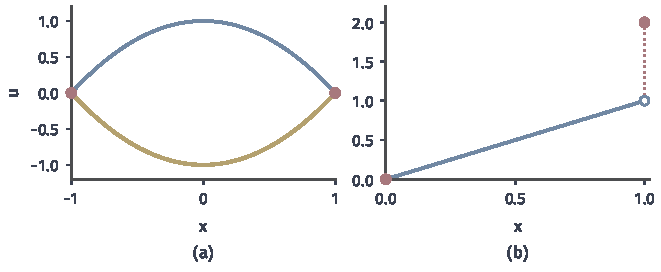
\includegraphics[width=112mm]{figures/06-differential-equations/02-partial-differential-equations/matplotlib/hj-boundary-failures/figure.pdf}
  \caption{边值问题的两种失败。(a)$\lvert u'\rvert=2\lvert x\rvert$，$u(\pm1)=0$（红点）有两个经典解$1-x^2$（蓝）和$x^2-1$（黄）。(b)$\lvert u'\rvert=1$，$u(0)=0$，$u(1)=2$（红点）：连续解取$u=x$，在右端得到$u(1)=1$（空心点），边值$2$没有被达到。}
  \label{fig:hj-boundary-failures}
\end{BookInlineFigure}

边界数据不相容时，问题出在另一处。在$(0,1)$上取$\lvert u'\rvert=1$，$u(0)=0$，$u(1)=2$。方程要求$u$是$1$-Lipschitz的，$u(1)$不可能等于$2$。自然的候选是
\[
  u(x)=\min\{0+x,\ 2+(1-x)\}=x,
\]
它在$(0,1)$内是黏性解，但在右端取值$1$，边值$2$被丢掉了，见图~\ref{fig:hj-boundary-failures}(b)。这对应第~\ref{sec:hj-problem}节的相容性条件。边值问题的比较原理假定函数已经在边界上按要求比较，它并不保证任何数据都能取到。

初值问题不会出现边值丢失，这里的差别列在表~\ref{tab:hj-comparison-cases}中，一种情形的结论不能搬到另一种情形。

\begin{BookInlineTable}
  \centering
  \begin{tabular}{lll}
    \toprule
    & 初值问题 & 程函边值问题\\
    \midrule
    严格性来源 & 时间函数$\psi$ & 系数$\theta<1$与$n>0$\\
    比较的部位 & $t=0$，全空间 & 边界$\partial\Omega$\\
    无穷远的控制 & 有界性、$\delta\lVert\bm{x}\rVert_2^2$ & 有界区域\\
    数据的限制 & 有界且Lipschitz & 需要相容，否则边值丢失\\
    条件破坏时 & 爆破、非唯一 & $n$有零点时非唯一\\
    \bottomrule
  \end{tabular}
  \caption{初值问题与边值问题的比较原理。}
  \label{tab:hj-comparison-cases}
\end{BookInlineTable}

\section{Hopf--Lax表示}
\label{sec:hj-hopf-lax}

比较原理保证黏性解至多一个，存在性还没有解决。对只依赖梯度的凸Hamilton量，解可以显式写出来，而且公式直接解释了尖点处选了哪一支。

\paragraph{从特征线到极小化}
设$H=H(\bm{p})$是凸函数，并且\term{超线性增长}（superlinear growth），即
\begin{equation}
  \lim_{\lVert\bm{p}\rVert_2\to\infty}\frac{H(\bm{p})}{\lVert\bm{p}\rVert_2}=+\infty.
  \label{eq:hj-superlinear}
\end{equation}
由第~\ref{sec:hj-characteristics}节的特征方程组，特征线是直线，斜率$\bm{p}$不变，速度$\bm{q}=\nabla H(\bm{p})$。沿线值的增量$\langle\bm{p},\nabla H(\bm{p})\rangle-H(\bm{p})$可以只用$\bm{q}$表示。

这里要用到凸共轭：对凸函数$H$，定义
\begin{equation}
  L(\bm{q})=\sup_{\bm{p}\in\mathbb{R}^{d}}\bigl\{\langle\bm{p},\bm{q}\rangle-H(\bm{p})\bigr\}.
  \label{eq:hj-legendre}
\end{equation}
$H$在$\bm{p}$处可微且$\bm{q}=\nabla H(\bm{p})$时，上确界在$\bm{p}$处取到，因此$L(\bm{q})=\langle\bm{p},\bm{q}\rangle-H(\bm{p})$，恰好是沿特征线值的增长率。凸共轭的基本性质（下半连续的凸函数共轭两次回到自身）可参考\BookChapterRef{chap:duality}{卷五第18章“对偶问题”}。

超线性让事情变得简单。对任意$r>0$，取$\bm{p}=r\bm{q}/\lVert\bm{q}\rVert_2$代入式~\eqref{eq:hj-legendre}，得到
\[
  L(\bm{q})\geq r\lVert\bm{q}\rVert_2-\max_{\lVert\bm{p}\rVert_2=r}H(\bm{p}).
\]
所以$L$同样超线性增长；由式~\eqref{eq:hj-superlinear}，式~\eqref{eq:hj-legendre}中的上确界有限。$L$是有限的凸函数，因而连续，并且由Fenchel--Moreau定理$H=L^*$。

最常用的例子是$H(\bm{p})=\lVert\bm{p}\rVert_2^2/2$，它的共轭是$L(\bm{q})=\lVert\bm{q}\rVert_2^2/2$。

从$\bm{y}$出发、时间$t$内到达$\bm{x}$的特征线速度是$\bm{q}=(\bm{x}-\bm{y})/t$，所以它带来的值是$u_0(\bm{y})+tL(\bm{q})$。不同的$\bm{y}$给出不同的候选值，我们取最小的一个。

\begin{definition}[Hopf--Lax公式]
\label{def:hj-hopf-lax}
设$H$凸且超线性增长，$L=H^*$，$u_0$有界且$R$-Lipschitz。对$t>0$，定义
\begin{equation}
  u(\bm{x},t)=\min_{\bm{y}\in\mathbb{R}^{d}}\Bigl\{u_0(\bm{y})+tL\Bigl(\frac{\bm{x}-\bm{y}}{t}\Bigr)\Bigr\},
  \label{eq:hj-hopf-lax}
\end{equation}
并令$u(\cdot,0)=u_0$。式~\eqref{eq:hj-hopf-lax}称为\term{Hopf--Lax公式}（Hopf--Lax formula）。
\end{definition}

对$H=p^2/2$，公式写成
\[
  u(x,t)=\min_y\Bigl\{u_0(y)+\frac{(x-y)^2}{2t}\Bigr\}.
\]
它有一个直观的图景，见图~\ref{fig:hj-parabola-touch}。把开口向下、顶点在$(x,c)$的抛物线$c-(x-y)^2/(2t)$放在$u_0$的下方，向上抬，直到碰到$u_0$，此时的$c$就是$u(x,t)$。接触点$y$是极小点，也就是这个位置的解“来自”的初始点。

\begin{BookInlineFigure}
  \centering
  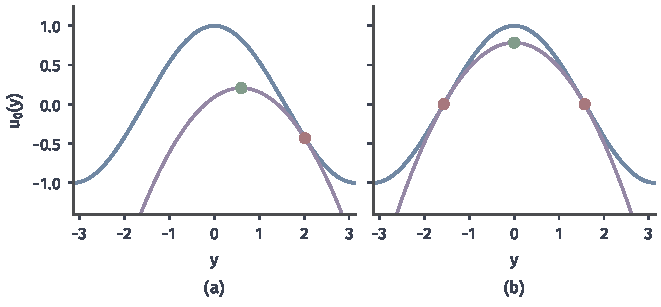
\includegraphics[width=112mm]{figures/06-differential-equations/02-partial-differential-equations/matplotlib/hj-parabola-touch/figure.pdf}
  \caption{Hopf--Lax公式的抛物线图景，$u_0=\cos y$（蓝），$t=\pi/2$。紫线是抬到碰上$u_0$为止的抛物线，绿点是顶点$(x,u(x,t))$，红点是接触点。(a)$x=0.6$，只有一个接触点。(b)$x=0$，两个接触点$y=\pm\pi/2$，顶点高度$\pi/4$。}
  \label{fig:hj-parabola-touch}
\end{BookInlineFigure}

\paragraph{公式的性质}
要证明式~\eqref{eq:hj-hopf-lax}给出黏性解，需要它的四条性质。最关键的一条是半群性质：走$t$时间等于先走$s$，再走$t-s$。

\begin{lemma}[Hopf--Lax公式的性质]
\label{lem:hj-hopf-lax}
在定义~\ref{def:hj-hopf-lax}的条件下：

(1)式~\eqref{eq:hj-hopf-lax}的极小值可以取到。

(2)$u(\cdot,t)$是$R$-Lipschitz的。

(3)对$0\leq s<t$，
\begin{equation}
  u(\bm{x},t)=\min_{\bm{y}}\Bigl\{u(\bm{y},s)+(t-s)L\Bigl(\frac{\bm{x}-\bm{y}}{t-s}\Bigr)\Bigr\}.
  \label{eq:hj-semigroup}
\end{equation}

(4)记
\begin{equation}
  C=\max\Bigl\{\lvert L(\bm{0})\rvert,\ \max_{\lVert\bm{p}\rVert_2\leq R}\lvert H(\bm{p})\rvert\Bigr\},
  \label{eq:hj-time-constant}
\end{equation}
则对$0\leq s\leq t$，
\begin{equation}
  \lvert u(\bm{x},t)-u(\bm{x},s)\rvert\leq C(t-s).
  \label{eq:hj-time-lipschitz}
\end{equation}
\end{lemma}

\begin{proof}
(1)括号内是$\bm{y}$的连续函数。$u_0$有界，$L$超线性增长，所以当$\lVert\bm{y}\rVert_2\to\infty$时括号内趋于$+\infty$，极小值可取到。

(2)设$\bm{y}$是$(\bm{x},t)$的极小点。把$\bm{y}+\hat{\bm{x}}-\bm{x}$代入$(\hat{\bm{x}},t)$的公式，$L$的自变量不变，所以
\[
  u(\hat{\bm{x}},t)-u(\bm{x},t)\leq u_0(\bm{y}+\hat{\bm{x}}-\bm{x})-u_0(\bm{y})\leq R\lVert\hat{\bm{x}}-\bm{x}\rVert_2.
\]
交换$\bm{x}$和$\hat{\bm{x}}$得到另一半。

(3)$s=0$时就是定义。设$s>0$。先证式中右端不超过左端。设$\bm{z}$是$(\bm{x},t)$的极小点，取线段上的点$\bm{y}=\frac{s}{t}\bm{x}+(1-\frac{s}{t})\bm{z}$，此时
\[
  \frac{\bm{x}-\bm{y}}{t-s}=\frac{\bm{y}-\bm{z}}{s}=\frac{\bm{x}-\bm{z}}{t}.
\]
用$u(\bm{y},s)\leq u_0(\bm{z})+sL((\bm{y}-\bm{z})/s)$，右端括号内不超过$u_0(\bm{z})+tL((\bm{x}-\bm{z})/t)=u(\bm{x},t)$。

再证左端不超过右端。任取$\bm{y}$，设$\bm{z}$是$(\bm{y},s)$的极小点。由$L$的凸性，
\[
  tL\Bigl(\frac{\bm{x}-\bm{z}}{t}\Bigr)\leq(t-s)L\Bigl(\frac{\bm{x}-\bm{y}}{t-s}\Bigr)+sL\Bigl(\frac{\bm{y}-\bm{z}}{s}\Bigr).
\]
再由$u(\bm{x},t)$的定义，得到
\[
  u(\bm{x},t)\leq u_0(\bm{z})+tL\Bigl(\frac{\bm{x}-\bm{z}}{t}\Bigr)\leq u(\bm{y},s)+(t-s)L\Bigl(\frac{\bm{x}-\bm{y}}{t-s}\Bigr).
\]

(4)先证$s=0$。上界由$\bm{y}=\bm{x}$得到：$u(\bm{x},t)\leq u_0(\bm{x})+tL(\bm{0})$。下界用$\bm{z}=(\bm{x}-\bm{y})/t$改写公式，再用Lipschitz条件：
\[
  u(\bm{x},t)\geq u_0(\bm{x})+t\min_{\bm{z}}\bigl\{L(\bm{z})-R\lVert\bm{z}\rVert_2\bigr\}.
\]
而$R\lVert\bm{z}\rVert_2$等于$\langle\bm{p},\bm{z}\rangle$在$\lVert\bm{p}\rVert_2\leq R$上的最大值。交换两个$\max$并用$H=L^*$，得到
\[
  -\min_{\bm{z}}\bigl\{L(\bm{z})-R\lVert\bm{z}\rVert_2\bigr\}=\max_{\lVert\bm{p}\rVert_2\leq R}H(\bm{p})\leq C.
\]
一般的$s$由式~\eqref{eq:hj-semigroup}和(2)，把$u(\cdot,s)$当作新的初值重复这一论证。
\end{proof}

\begin{theorem}[Hopf--Lax公式给出黏性解]
\label{thm:hj-hopf-lax}
在定义~\ref{def:hj-hopf-lax}的条件下，式~\eqref{eq:hj-hopf-lax}定义的$u$在任意$\mathbb{R}^{d}\times[0,t_{\mathrm{f}}]$上有界、Lipschitz，是初值问题$\partial_tu+H(\nabla u)=0$、$u(\cdot,0)=u_0$的黏性解，并且是有界、一致连续、关于$\bm{x}$为$R$-Lipschitz的函数类中唯一的黏性解。
\end{theorem}

\begin{proof}
由引理~\ref{lem:hj-hopf-lax}，$u$有界，界为$\sup\lvert u_0\rvert+Ct_{\mathrm{f}}$；$u$关于$\bm{x}$是$R$-Lipschitz的，关于$t$是$C$-Lipschitz的，$t=0$时取值$u_0$。

\emph{次解。}设$u-\varphi$在$(\bm{x}_0,t_0)$取局部极大，$t_0>0$。任取$\bm{q}$和小$h>0$，在式~\eqref{eq:hj-semigroup}中取$\bm{y}=\bm{x}_0-h\bm{q}$、$s=t_0-h$，得到
\[
  u(\bm{x}_0,t_0)\leq u(\bm{x}_0-h\bm{q},t_0-h)+hL(\bm{q}).
\]
由局部极大，$u-\varphi$在$(\bm{x}_0-h\bm{q},t_0-h)$处不大于在$(\bm{x}_0,t_0)$处，整理后得到
\[
  \varphi(\bm{x}_0,t_0)-\varphi(\bm{x}_0-h\bm{q},t_0-h)\leq hL(\bm{q}).
\]
除以$h$，令$h\to0$，得到
\[
  \partial_t\varphi+\langle\bm{q},\nabla\varphi\rangle-L(\bm{q})\leq0.
\]
对$\bm{q}$取上确界并用$H=L^*$，得到$\partial_t\varphi+H(\nabla\varphi)\leq0$。

\emph{上解。}设$u-\varphi$在$(\bm{x}_0,t_0)$取局部极小。由式~\eqref{eq:hj-semigroup}（取$s=t_0-h$）和(1)，存在$\bm{y}_h$，记$\bm{q}_h=(\bm{x}_0-\bm{y}_h)/h$，使
\[
  u(\bm{x}_0,t_0)=u(\bm{y}_h,t_0-h)+hL(\bm{q}_h).
\]
由$u$的Lipschitz性质，$hL(\bm{q}_h)\leq Rh\lVert\bm{q}_h\rVert_2+Ch$。$L$超线性增长，所以$\lVert\bm{q}_h\rVert_2$有不依赖$h$的上界。

由局部极小，同样整理得到
\[
  \varphi(\bm{x}_0,t_0)-\varphi(\bm{y}_h,t_0-h)\geq hL(\bm{q}_h).
\]
$\varphi\in C^1$且$\bm{q}_h$有界，所以左端等于$h(\partial_t\varphi+\langle\bm{q}_h,\nabla\varphi\rangle)+o(h)$，其中导数在$(\bm{x}_0,t_0)$处取值。除以$h$，得到
\[
  \partial_t\varphi+\langle\bm{q}_h,\nabla\varphi\rangle-L(\bm{q}_h)\geq o(1).
\]
由Fenchel--Young不等式（$H=L^*$的定义），左端第二、三两项不超过$H(\nabla\varphi)$。令$h\to0$，得到$\partial_t\varphi+H(\nabla\varphi)\geq0$。

\emph{唯一性。}$H$连续，在$\lVert\bm{p}\rVert_2\leq R$上一致连续，由定理~\ref{thm:hj-uniqueness}即得。
\end{proof}

证明的结构和方程的含义一一对应：极小化的上界对应每一条候选路线都给出不等式，所以次解成立；极小化取到的那条路线给出反向的不等式，所以上解成立。

\paragraph{公式怎样选择分支}
回到$u_0=\cos x$，取$t=\pi/2$、$x=0$。极小化的函数是$F(y)=\cos y+y^2/\pi$，临界点方程是
\[
  F'(y)=-\sin y+\frac{2y}{\pi}=0,
\]
即$\sin y=2y/\pi$。由$\sin$在$[0,\pi]$上的凹性，它的非负解只有$y=0$和$y=\pi/2$；再由对称性，全部解是$y=0,\pm\pi/2$。代入$F$得到
\[
  F(0)=1,\qquad F\bigl(\pm\tfrac{\pi}{2}\bigr)=\frac{\pi}{4}\approx0.785.
\]
所以$u(0,\pi/2)=\pi/4$，极小点是$y=\pm\pi/2$。这三个临界点恰好是第~\ref{sec:hj-cusps}节算出的三条特征线，函数值也与当时的$z$相同。

这个吻合有一般的原因。设$u_0$、$L$、$H$可微，$\bm{q}$表示$(\bm{x}-\bm{y})/t$，极小点满足一阶条件$\nabla u_0(\bm{y})=\nabla L(\bm{q})$。由共轭函数的性质，这等价于$\bm{q}$等于$\nabla H$在$\bm{p}_0=\nabla u_0(\bm{y})$处的值，也就是
\[
  \bm{x}=\bm{y}+t\nabla H(\bm{p}_0).
\]
所以每个临界点都对应一条到达$(\bm{x},t)$的特征线，临界值就是这条线带来的$z$。Hopf--Lax公式在所有特征线中选择取值最小的一条，这回答了第~\ref{sec:hj-cusps}节的问题：对凸的$H$，黏性解取的就是所有特征线候选的下包络。

图~\ref{fig:hj-argmin-jump}(a)是目标函数$F$。$x=0$时两个极小点等高；$x=0.3$时右侧变低，唯一的极小点约为$y=1.822$，极小值$0.489$。图(b)是极小点随$x$的变化，在$x=0$处从$-\pi/2$跳到$\pi/2$，这个跳跃就是图~\ref{fig:hj-cos-characteristics}(b)中两族特征线之间的分界。

\begin{BookInlineFigure}
  \centering
  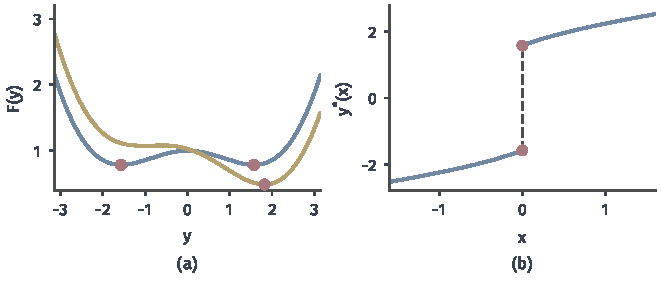
\includegraphics[width=112mm]{figures/06-differential-equations/02-partial-differential-equations/matplotlib/hj-argmin-jump/figure.pdf}
  \caption{极小点的跳跃，$t=\pi/2$，$F(y)=\cos y+(x-y)^2/(2t)$。(a)$x=0$（蓝）有两个等高的极小点，$x=0.3$（黄）只有一个，红点是极小点。(b)极小点$y^*(x)$，虚线处从$-\pi/2$跳到$\pi/2$。}
  \label{fig:hj-argmin-jump}
\end{BookInlineFigure}

\begin{theorem}[极小点决定梯度]
\label{thm:hj-minimizer-gradient}
设$L$连续可微，$\bm{y}$是$(\bm{x},t)$的一个极小点，$t>0$。若$u(\cdot,t)$在$\bm{x}$处可微，则
\begin{equation}
  \nabla u(\bm{x},t)=\nabla L\Bigl(\frac{\bm{x}-\bm{y}}{t}\Bigr).
  \label{eq:hj-minimizer-gradient}
\end{equation}
特别地，若$L$还是严格凸的，而$(\bm{x},t)$有两个不同的极小点，则$u(\cdot,t)$在$\bm{x}$处不可微。
\end{theorem}

\begin{proof}
对任意$\bm{x}'$，$\bm{y}$仍是公式的一个候选，所以
\[
  u(\bm{x}',t)\leq u_0(\bm{y})+tL\Bigl(\frac{\bm{x}'-\bm{y}}{t}\Bigr),
\]
且$\bm{x}'=\bm{x}$时取等。右端是$\bm{x}'$的$C^1$函数，从上方贴住$u(\cdot,t)$，一阶条件给出式~\eqref{eq:hj-minimizer-gradient}。

若有两个极小点，$(\bm{x}-\bm{y})/t$取两个不同的值，严格凸函数的梯度是单射，式~\eqref{eq:hj-minimizer-gradient}的右端不同，矛盾。
\end{proof}

不可微点就是多个极小点的位置，也就是特征线竞争时打平的位置。在$x=0$、$t=\pi/2$，两个极小点给出$q=(0\mp\pi/2)/(\pi/2)=\mp1$，$u$的左斜率是$+1$，右斜率是$-1$，形成凹折角。

折角只会是凹的，这一点可以直接证明。对$H=\lVert\bm{p}\rVert_2^2/2$，公式展开平方，得到
\[
  u(\bm{x},t)-\frac{\lVert\bm{x}\rVert_2^2}{2t}=\min_{\bm{y}}\Bigl\{u_0(\bm{y})+\frac{\lVert\bm{y}\rVert_2^2}{2t}-\frac{\langle\bm{x},\bm{y}\rangle}{t}\Bigr\}.
\]
右端是$\bm{x}$的仿射函数的极小，所以是凹函数。这种减去二次函数后变成凹函数的性质叫做\term{半凹}（semiconcave）。它排除了$t>0$时的一切凸折角。

一维时，这条性质说$\partial_xu-x/t$不增，即$v=\partial_xu$对$a>0$满足$v(x+a)-v(x)\leq a/t$。这就是Burgers方程熵解的单侧增长界（Oleinik条件），也说明了凹槽$w$的底部为何从一开始就被排除。

\paragraph{两种折角的算例}
把$u_0=\pm\lvert x\rvert$代入公式，可以完整地手算，取$H=p^2/2$。

对$u_0=\lvert x\rvert$，先在$y>0$上求极小：$1+(y-x)/t=0$，得$y=x-t$，要求$x>t$，此时值为$x-t/2$。$y<0$的情形对称。其余情况极小点在折角$y=0$处，值为$x^2/(2t)$。汇总得
\begin{equation}
  u(x,t)=\begin{cases}x^2/(2t),&\lvert x\rvert\leq t,\\\lvert x\rvert-t/2,&\lvert x\rvert>t.\end{cases}
  \label{eq:hj-convex-kink}
\end{equation}
初值的凸折角立刻被抹平。$\partial_xu=x/t$，正是第~\ref{chap:scalar-conservation-laws}章的稀疏波。

对$u_0=-\lvert x\rvert$，在$y>0$上一阶条件$-1+(y-x)/t=0$给出$y=x+t$，值$-x-t/2$；在$y<0$上$y=x-t$，值$x-t/2$。比较两者取较小，得到
\begin{equation}
  u(x,t)=-\lvert x\rvert-\frac{t}{2}.
  \label{eq:hj-concave-kink}
\end{equation}
凹折角一直存在，$x=0$上$v$的跳跃是激波。图~\ref{fig:hj-fan-kink}是两种情形的对比。

\begin{BookInlineFigure}
  \centering
  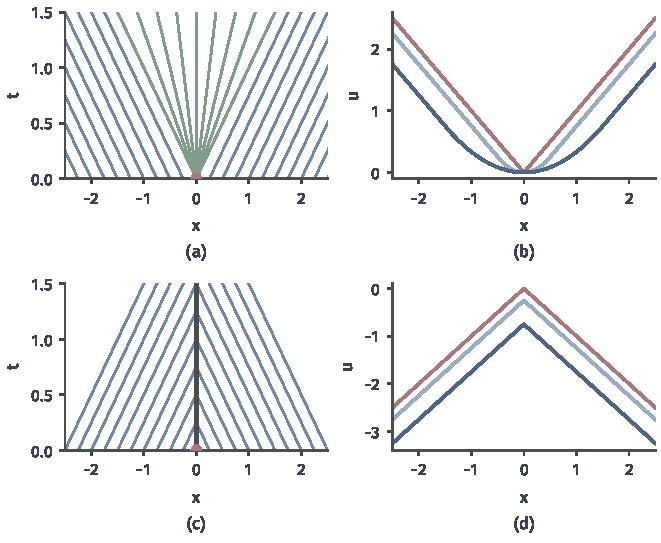
\includegraphics[width=112mm]{figures/06-differential-equations/02-partial-differential-equations/matplotlib/hj-fan-kink/figure.pdf}
  \caption{$H=p^2/2$下两种折角的演化。(a)、(b)$u_0=\lvert x\rvert$：折角处发出绿色扇形特征线填补空隙，解由式~\eqref{eq:hj-convex-kink}给出。(c)、(d)$u_0=-\lvert x\rvert$：蓝色特征线都汇入深灰的折角线，解由式~\eqref{eq:hj-concave-kink}给出。(b)、(d)中红线是初值，蓝色由浅到深是$t=0.5,1.5$。}
  \label{fig:hj-fan-kink}
\end{BookInlineFigure}

\paragraph{条件的作用}
凸性不能省略。公式只依赖$L=H^*$，而不同的$H$可能有相同的$L$。由Fenchel--Moreau定理，$L^*$是$H$的闭凸包，所以式~\eqref{eq:hj-hopf-lax}求解的其实是$H^{**}$对应的方程。若$H$不凸，$H^{**}\neq H$，公式给出的就不是原方程的解。

初值有界也用到了。对$u_0=-x^2/2$、$H=p^2/2$和$t>1$，公式中的目标函数
\[
  -\frac{y^2}{2}+\frac{(x-y)^2}{2t}
\]
的二次项系数是$\frac{1}{2t}-\frac12<0$，下确界是$-\infty$，公式失去意义。这和上一节经典解在$t=1$爆破是一致的。

\paragraph{到达时间：极限情形}
波前对应$H(\bm{p})=\lVert\bm{p}\rVert_2$，它是凸的，但只线性增长。此时共轭函数是单位球的指示函数：$\lVert\bm{q}\rVert_2\leq1$时$L(\bm{q})=0$，否则$L=+\infty$。把它代入式~\eqref{eq:hj-hopf-lax}，得到
\begin{equation}
  u(\bm{x},t)=\min_{\lVert\bm{y}-\bm{x}\rVert_2\leq t}u_0(\bm{y}).
  \label{eq:hj-erosion}
\end{equation}
定理~\ref{thm:hj-hopf-lax}不直接覆盖这种情形，但它的证明可以照搬：极小点在紧球上取得，半群性质只用到$L$的凸性，$\bm{q}_h$在单位球内，有界性不用再证，$H=L^*$仍然成立。所以式~\eqref{eq:hj-erosion}是有界Lipschitz初值下的黏性解。

这个公式说，$u$在$(\bm{x},t)$的值是初值在半径$t$的球内的最小值。取一个闭的源集$S$，$u_0=d(\cdot,S)$是到$S$的距离（要满足有界性，可以在远处截断，有限时间内的结果不受影响）。则
\[
  u(\bm{x},t)=\max\{d(\bm{x},S)-t,\ 0\},
\]
所以$\{u(\cdot,t)=0\}=\{d(\cdot,S)\leq t\}$恰好是时刻$t$已被扫过的区域，到达时间$T=d(\cdot,S)$从解中读出。

图~\ref{fig:hj-erosion}取一维的$S=\{-1.5,1\}$。相向的两列波前在$x=-0.25$、时刻$1.25$相遇，这正是图(b)的折角点。这与定理~\ref{thm:hj-distance}的结论一致，$T$就是到$S$的距离。

\begin{BookInlineFigure}
  \centering
  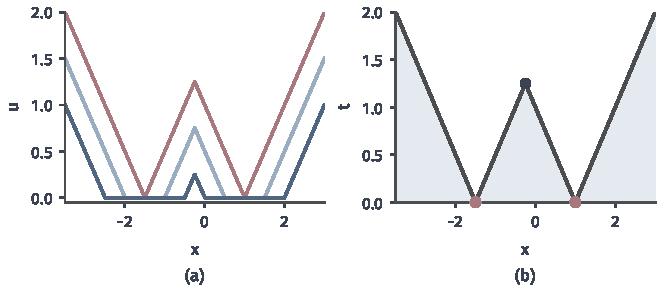
\includegraphics[width=112mm]{figures/06-differential-equations/02-partial-differential-equations/matplotlib/hj-erosion/figure.pdf}
  \caption{$H=\lvert p\rvert$的极限情形。(a)初值$u_0=d(x,S)$（红），$S=\{-1.5,1\}$，蓝色由浅到深是$t=0.5,1$的解，零值区域在扩大。(b)$(x,t)$平面，红点是源，深灰线是$T(x)=d(x,S)$，也就是四条波前的轨迹，浅蓝是波前尚未到达的区域$t<T(x)$，黑点$(-0.25,1.25)$是两列波前相遇的位置。}
  \label{fig:hj-erosion}
\end{BookInlineFigure}

Hopf--Lax公式的外形是在速度和代价之间做选择，让人想到控制问题。这一节只把它用作方程的表示公式：$L$由$H$算出来，极小化的作用是从特征线中选出黏性解。本章不需要问谁在做决策，也不需要讨论最优策略是否存在。

\section{消失黏性}
\label{sec:hj-vanishing}

第~\ref{chap:pde-problems}章已经见过，给程函方程加一个小扩散项，解的极限就是到边界的距离。这一节解释这个现象：在方程中加入$\varepsilon\Delta u$，光滑解在$\varepsilon\to0$时为什么收敛到黏性解，以及有限的$\varepsilon$下误差有多大。

考虑带小扩散的方程
\begin{equation}
  \partial_tu_\varepsilon+H(\nabla u_\varepsilon)=\varepsilon\Delta u_\varepsilon,\qquad u_\varepsilon(\cdot,0)=u_0,
  \label{eq:hj-viscous}
\end{equation}
其中$\varepsilon>0$。$\varepsilon$前面的符号与第~\ref{chap:diffusion-equations}章的热方程相同，时间向前是适定的。

\paragraph{一个可以精确求解的例子}
对$H=\lVert\bm{p}\rVert_2^2/2$，式~\eqref{eq:hj-viscous}可以化成线性的热方程。设$u_\varepsilon=-2\varepsilon\ln w$，$w>0$，这称为\term{Cole--Hopf变换}（Cole--Hopf transformation）。分别计算各项：
\[
  \partial_tu_\varepsilon=-2\varepsilon\frac{\partial_tw}{w},\qquad
  \frac12\lVert\nabla u_\varepsilon\rVert_2^2=2\varepsilon^2\frac{\lVert\nabla w\rVert_2^2}{w^2}.
\]
Laplace项为
\[
  \varepsilon\Delta u_\varepsilon=-2\varepsilon^2\frac{\Delta w}{w}+2\varepsilon^2\frac{\lVert\nabla w\rVert_2^2}{w^2}.
\]
代入式~\eqref{eq:hj-viscous}，含$\lVert\nabla w\rVert_2^2$的两项抵消，非线性消失了，剩下
\[
  \partial_tw=\varepsilon\Delta w.
\]

由第~\ref{chap:diffusion-equations}章的热核表示，$\partial_tw=\varepsilon\Delta w$在全空间的有界解是初值与Gauss核的卷积，初值取$w_0=\mathrm{e}^{-u_0/(2\varepsilon)}$。两个指数的自变量合并后，正好出现Hopf--Lax公式中的函数。记
\[
  F(\bm{y})=u_0(\bm{y})+\frac{\lVert\bm{x}-\bm{y}\rVert_2^2}{2t},
\]
则
\begin{equation}
  u_\varepsilon(\bm{x},t)=-2\varepsilon\ln\Bigl[(4\pi\varepsilon t)^{-d/2}\int_{\mathbb{R}^{d}}\mathrm{e}^{-F(\bm{y})/(2\varepsilon)}\,\mathrm{d}\bm{y}\Bigr].
  \label{eq:hj-cole-hopf}
\end{equation}

式~\eqref{eq:hj-cole-hopf}是一个“软极小”。图~\ref{fig:hj-cole-hopf-softmin}是$(x,t)=(0,\pi/2)$时的被积函数：$\varepsilon$变小时，权重集中到$F$的两个极小点附近，$-2\varepsilon\ln$把积分的值换算回$F$的尺度。

\begin{BookInlineFigure}
  \centering
  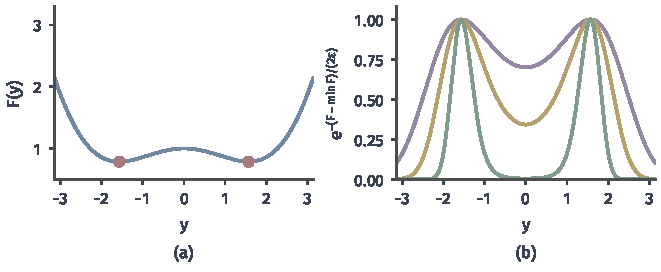
\includegraphics[width=112mm]{figures/06-differential-equations/02-partial-differential-equations/matplotlib/hj-cole-hopf-softmin/figure.pdf}
  \caption{Cole--Hopf公式中的权重，$u_0=\cos y$，$(x,t)=(0,\pi/2)$。(a)$F(y)$，红点是两个极小点。(b)归一化的被积函数，$\varepsilon=0.3$（紫）、$0.1$（黄）、$0.02$（绿）。$\varepsilon$变小时质量集中到极小点。}
  \label{fig:hj-cole-hopf-softmin}
\end{BookInlineFigure}

\begin{theorem}[Cole--Hopf解的极限]
\label{thm:hj-cole-hopf-limit}
设$u_0$有界且$R$-Lipschitz，$H=\lVert\bm{p}\rVert_2^2/2$，$u$是式~\eqref{eq:hj-hopf-lax}。对任意$0<t_1<t_2$，存在常数$C$，使对$t\in[t_1,t_2]$、$\bm{x}\in\mathbb{R}^{d}$和$0<\varepsilon\leq1/2$，
\begin{equation}
  \lvert u_\varepsilon(\bm{x},t)-u(\bm{x},t)\rvert\leq C\varepsilon\ln\frac{1}{\varepsilon}.
  \label{eq:hj-cole-hopf-limit}
\end{equation}
\end{theorem}

\begin{proof}
记$m=\min F=u(\bm{x},t)$，$M=\sup\lvert u_0\rvert$，$\bm{y}^*$为一个极小点。由$F(\bm{x})\leq M$，得$m\leq M$。

先估计积分的上界。由$u_0\geq-M$，得到
\[
  F(\bm{y})\geq-M+\frac{\lVert\bm{x}-\bm{y}\rVert_2^2}{2t}.
\]
取$\rho^2=8Mt$，当$\lVert\bm{x}-\bm{y}\rVert_2\geq\rho$时，
\[
  F(\bm{y})-m\geq\frac{\lVert\bm{x}-\bm{y}\rVert_2^2}{2t}-2M\geq\frac{\lVert\bm{x}-\bm{y}\rVert_2^2}{4t}.
\]
球内用$F\geq m$。合起来，记$\lvert B_\rho\rvert$为半径$\rho$的球的体积，得
\[
  \int\mathrm{e}^{-F/(2\varepsilon)}\,\mathrm{d}\bm{y}\leq\mathrm{e}^{-m/(2\varepsilon)}\bigl(\lvert B_\rho\rvert+(8\pi\varepsilon t)^{d/2}\bigr).
\]

再估计下界。由$\rho$的取法，极小点满足$\lVert\bm{x}-\bm{y}^*\rVert_2\leq\rho$。在$\bm{y}^*$的半径$\varepsilon$的球内，$F$是$\Lambda$-Lipschitz的，$\Lambda=R+(\rho+1)/t$，所以$F\leq m+\Lambda\varepsilon$，积分至少是
\[
  \mathrm{e}^{-m/(2\varepsilon)}\mathrm{e}^{-\Lambda/2}\lvert B_\varepsilon\rvert.
\]

把这两个界代入式~\eqref{eq:hj-cole-hopf}，$-2\varepsilon\ln$作用在$\mathrm{e}^{-m/(2\varepsilon)}$上得到$m$，其余因子是$\varepsilon$的幂次和$t\in[t_1,t_2]$上有界的常数，它们取对数再乘$2\varepsilon$后，不超过$C\varepsilon\ln(1/\varepsilon)$。
\end{proof}

所以在这个模型中，消失黏性的极限就是Hopf--Lax公式，也就是唯一的黏性解。

折角附近的结构也能精确算出。在$(0,\pi/2)$附近，$F$有两个极小点$\pm\pi/2$，$F''(\pm\pi/2)=2/\pi$，也就是$tF''=1$。把积分在两个极小点附近用Gauss积分近似，每个贡献$\sqrt{4\pi\varepsilon/F''}\,\mathrm{e}^{-\pi/(8\varepsilon)}$，于是
\begin{equation}
  u_\varepsilon(0,\pi/2)=\frac{\pi}{4}-2\varepsilon\ln2+O(\varepsilon^2).
  \label{eq:hj-kink-correction}
\end{equation}
其中$\ln2$来自“两个极小点”。表~\ref{tab:hj-kink-correction}用式~\eqref{eq:hj-cole-hopf}的数值积分核对，$\varepsilon$越小吻合得越好。

\begin{BookInlineTable}
  \centering
  \begin{tabular}{cccc}
    \toprule
    $\varepsilon$ & $0.2$ & $0.05$ & $0.01$\\
    \midrule
    $\pi/4-u_\varepsilon(0,\pi/2)$ & $0.2842$ & $0.0800$ & $0.0142$\\
    $2\varepsilon\ln2$ & $0.2773$ & $0.0693$ & $0.0139$\\
    \bottomrule
  \end{tabular}
  \caption{折角处的黏性修正，$u_0=\cos x$，$H=p^2/2$。}
  \label{tab:hj-kink-correction}
\end{BookInlineTable}

两条分支在$x=0$附近可以近似写成$\pi/4\pm x$，软极小给出
\[
  u_\varepsilon\approx\frac{\pi}{4}-2\varepsilon\ln\Bigl(2\cosh\frac{x}{2\varepsilon}\Bigr),\qquad
  \partial_xu_\varepsilon\approx-\tanh\frac{x}{2\varepsilon}.
\]
折角被抹成宽度约$\varepsilon$的过渡层，它的斜率恰好是第~\ref{chap:scalar-conservation-laws}章Burgers方程的黏性激波剖面。图~\ref{fig:hj-viscous-limit}显示这个过程。

\begin{BookInlineFigure}
  \centering
  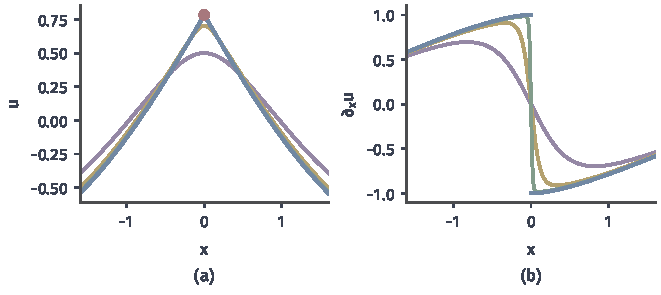
\includegraphics[width=112mm]{figures/06-differential-equations/02-partial-differential-equations/matplotlib/hj-viscous-limit/figure.pdf}
  \caption{消失黏性的极限，$u_0=\cos x$，$t=\pi/2$。(a)式~\eqref{eq:hj-cole-hopf}的$u_\varepsilon$，$\varepsilon=0.2$（紫）、$0.05$（黄）、$0.01$（绿），蓝线是Hopf--Lax解，红点是折角。(b)对应的斜率，$\varepsilon$变小时过渡层变窄，趋向蓝线在$x=0$的跳跃。}
  \label{fig:hj-viscous-limit}
\end{BookInlineFigure}

到达时间也有同样的线性化。令$T_\varepsilon=-\varepsilon\ln w$，代入带小扩散的方程
\[
  \lVert\nabla T_\varepsilon\rVert_2^2-\varepsilon\Delta T_\varepsilon=1,
\]
得到线性方程
\[
  \varepsilon^2\Delta w=w.
\]
第~\ref{chap:pde-problems}章的一维显式解就是$w=\cosh(x/\varepsilon)/\cosh(1/\varepsilon)$。

在平面上，点源的径向解是修正Bessel函数$K_0(r/\varepsilon)$，它满足$\varepsilon^2\Delta w=w$（$r>0$）。两个源的线性叠加给出
\[
  T_\varepsilon=-\varepsilon\ln\Bigl[K_0\bigl(\lVert\bm{x}-\bm{a}\rVert_2/\varepsilon\bigr)+K_0\bigl(\lVert\bm{x}-\bm{b}\rVert_2/\varepsilon\bigr)\Bigr].
\]
$K_0(z)$随$z$增大以$\mathrm{e}^{-z}$的速度衰减，所以$T_\varepsilon$是两个距离的软极小。图~\ref{fig:hj-soft-two-sources}显示，$\varepsilon$变小时，等值线向$T=\min\{T_1,T_2\}$靠拢，中垂线上的尖角由圆滑变尖锐。

\begin{BookInlineFigure}
  \centering
  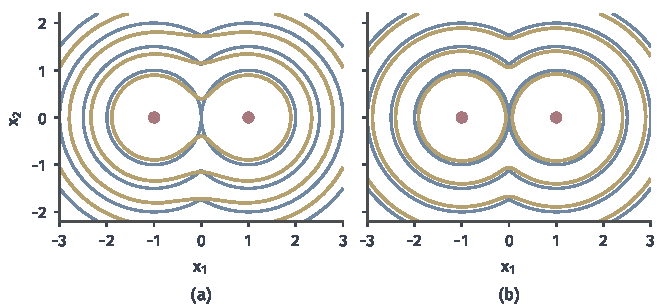
\includegraphics[width=112mm]{figures/06-differential-equations/02-partial-differential-equations/matplotlib/hj-soft-two-sources/figure.pdf}
  \caption{到达时间的软化，源为两个红点。蓝线是$T=\min\{T_1,T_2\}$的等值线$1,1.5,2,2.5$，黄线是$T_\varepsilon$的相同等值线。(a)$\varepsilon=0.3$。(b)$\varepsilon=0.08$。}
  \label{fig:hj-soft-two-sources}
\end{BookInlineFigure}

\paragraph{一般Hamilton量}
一般的$H$没有线性化，但结论不依赖显式解，其根据是黏性解在局部一致极限下稳定。

\begin{theorem}[黏性解的稳定性]
\label{thm:hj-stability-viscosity}
设$H$连续，$u_\varepsilon\in C^2$是式~\eqref{eq:hj-viscous}中方程的经典解，$\varepsilon\to0$时$u_\varepsilon\to u$在$\mathbb{R}^{d}\times(0,t_{\mathrm{f}})$上局部一致成立。则$u$是
\begin{equation}
  \partial_tu+H(\nabla u)=0
  \label{eq:hj-limit-equation}
\end{equation}
的黏性解。
\end{theorem}

\begin{proof}
只证次解，上解同理。设$\varphi\in C^1$，$u-\varphi$在$P$取局部极大。换成$\tilde\varphi=\varphi+\lVert\bm{z}-P\rVert_2^2$（$\bm{z}=(\bm{x},t)$），它在$P$的导数不变，且$u-\tilde\varphi$在$P$取严格局部极大。取以$P$为中心的闭球$B$，$B$在$t>0$内，使$P$是$u-\tilde\varphi$在$B$上唯一的最大点。

取光滑函数$\varphi^\eta$在$B$上连同一阶导数一致收敛到$\tilde\varphi$。固定$\eta$，$u_\varepsilon-\varphi^\eta$在$B$上的最大点记为$P_{\varepsilon}$。当它在$B$的内部时，一阶和二阶条件给出
\[
  \partial_t\varphi^\eta(P_\varepsilon)+H\bigl(\nabla\varphi^\eta(P_\varepsilon)\bigr)=\varepsilon\Delta u_\varepsilon(P_\varepsilon)\leq\varepsilon\Delta\varphi^\eta(P_\varepsilon).
\]

$\varphi^\eta$是固定的光滑函数，$\Delta\varphi^\eta$在$B$上有界。由一致收敛，$\varepsilon\to0$时$P_\varepsilon$的聚点是$u-\varphi^\eta$在$B$上的最大点；$\eta$充分小时这些点都靠近$P$，从而在$B$内部。令$\varepsilon\to0$，得到在某个最大点$P^\eta$处
\[
  \partial_t\varphi^\eta(P^\eta)+H\bigl(\nabla\varphi^\eta(P^\eta)\bigr)\leq0.
\]
再令$\eta\to0$，$P^\eta\to P$，$\varphi^\eta$的导数收敛到$\tilde\varphi$的导数，由$H$的连续性得到$\partial_t\varphi(P)+H(\nabla\varphi(P))\leq0$。
\end{proof}

证明只用到局部一致收敛，这就是黏性解在极限下稳定的原因。不需要梯度的强收敛，而对弱解来说，$H(\nabla u_\varepsilon)$的弱极限一般不是$H(\nabla u)$。

\begin{theorem}[消失黏性选择黏性解]
\label{thm:hj-vanishing-viscosity}
设$H$连续，$u_0$有界且$R$-Lipschitz。设对每个充分小的$\varepsilon$，式~\eqref{eq:hj-viscous}有$C^2$解$u_\varepsilon$，并且存在不依赖$\varepsilon$的常数$C$，使
\begin{equation}
  \lvert u_\varepsilon\rvert\leq C,\qquad\lVert\nabla u_\varepsilon\rVert_2\leq R,\qquad\lvert\partial_tu_\varepsilon\rvert\leq C.
  \label{eq:hj-uniform-estimates}
\end{equation}
则$\varepsilon\to0$时，$u_\varepsilon$局部一致收敛到初值问题唯一的有界、关于$\bm{x}$是$R$-Lipschitz的黏性解。
\end{theorem}

\begin{proof}
由式~\eqref{eq:hj-uniform-estimates}，$\{u_\varepsilon\}$一致有界且等度连续。由Arzel\`a--Ascoli定理，一致有界、等度连续的函数列在紧集上有一致收敛的子列。取任一收敛子列，极限$u$继承相同的界，由定理~\ref{thm:hj-stability-viscosity}是黏性解，$u(\cdot,0)=u_0$。

由定理~\ref{thm:hj-uniqueness}，这样的黏性解只有一个，所以所有收敛子列有相同的极限，整个族收敛。
\end{proof}

式~\eqref{eq:hj-uniform-estimates}是定理的条件，不是自动成立的。对光滑的$H(\bm{p})$，它们来自线性抛物方程的最大值原理：差商$u_\varepsilon(\bm{x}+\bm{h},t)-u_\varepsilon(\bm{x},t)$满足一个线性抛物方程，最大值在初始时刻取得，所以空间Lipschitz常数不增加，时间导数的界要求初值更光滑或先磨光初值。光滑解的存在性证明要用到抛物方程的正则性理论，篇幅较长，可查阅\scite{math-bardi1997hjb}。

所以$\varepsilon\Delta u$的作用和第~\ref{chap:scalar-conservation-laws}章在守恒律中的作用一样：它打破了对称，选择了一个解。$\varepsilon$的符号决定选哪个，这就是第~\ref{chap:pde-problems}章看到的符号问题。

\paragraph{有限黏性的误差}
$\varepsilon>0$时$u_\varepsilon$是光滑的，但它只是近似。一般的Lipschitz初值下，$\sup\lvert u_\varepsilon-u\rvert$的量级是$\sqrt{\varepsilon t}$，证明要用变量倍增并同时估计黏性项，篇幅较长，读者可查阅\scite{math-bardi1997hjb}。这个量级的含义是：在只有Lipschitz正则性时，误差随$\varepsilon$减小得比$\varepsilon$本身慢。在例~\ref{ex:hj-cos}中，由于解的结构特殊，$x=0$处的误差是$O(\varepsilon)$，见式~\eqref{eq:hj-kink-correction}和图~\ref{fig:hj-two-limits}(b)。

\paragraph{不要混淆两个极限}
实际计算时有两个参数：黏性$\varepsilon$和网格步长$h$。令$h\to0$只是更准确地解带$\varepsilon$的方程，令$\varepsilon\to0$才改变方程本身。

图~\ref{fig:hj-two-limits}(a)做了一个实验：固定$\varepsilon=0.1$，用周期网格上的中心差分和显式时间推进，时间步足够小，算到$t=\pi/2$。随着网格加密，到$u_\varepsilon$的误差按$h^2$下降，从$N=20$时的$0.056$降到$N=640$时的$6\times10^{-5}$。到$u$的误差却停在$0.159$附近，这是黏性解与带黏性方程的差，再细的网格也消除不了。

\begin{BookInlineFigure}
  \centering
  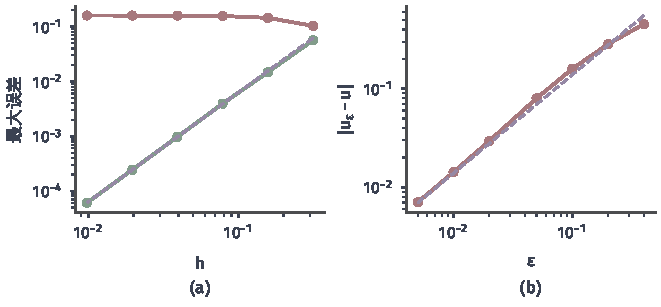
\includegraphics[width=112mm]{figures/06-differential-equations/02-partial-differential-equations/matplotlib/hj-two-limits/figure.pdf}
  \caption{两个极限的区分，$u_0=\cos x$，$t=\pi/2$。(a)固定$\varepsilon=0.1$，网格点数$N=20,\ldots,640$（$h=2\pi/N$），绿线是数值解到$u_\varepsilon$的最大误差，红线是到黏性解$u$的最大误差，紫色虚线是$h^2$的参考斜率。(b)式~\eqref{eq:hj-cole-hopf}在$x=0$处的误差随$\varepsilon$的变化，紫色虚线是$2\varepsilon\ln2$。}
  \label{fig:hj-two-limits}
\end{BookInlineFigure}

要逼近$u$本身，必须同时让$\varepsilon\to0$，并且让网格能够分辨宽度约$\varepsilon$的过渡层，或者在格式里内建适当的数值耗散。后一种做法把$\varepsilon$隐含在网格步长中，两个极限就合并了，这时收敛性需要专门的分析，不能从上面的实验推出。

\section{本章小结}
\label{sec:hj-summary}

本章围绕一个问题展开：当方程只限制局部的梯度时，场值由什么决定。到达时间给出了具体的图景，波前法向推进的速度决定$T$梯度的长度；令$u=T-t$，到达时间问题就进入时间依赖的方程，Hamilton量$H$说明斜率$\bm{p}$的地方高度下降多快。两类问题的数据不同，边值问题还要求数据相容。

光滑时，方程化为特征方程组。位置和斜率服从Hamilton方程，值靠一次积分带上，这样可以局部重建经典解。对波前而言，特征线就是射线，$u$沿线不变。

特征线会相交。一维中曲率按式~\eqref{eq:hj-riccati}发散，经典解在有限时刻结束，而斜率和场值依然有界。此后同一位置有多个候选，几乎处处满足方程的解不唯一，凹槽就是例子。

黏性解在接触点处提出不等式：从上方贴得到$\leq0$，从下方贴得到$\geq0$。它不做积分，也不移走导数，而且对方程的符号敏感。凹折角通过检验，凸折角不通过，这和“只有第一次到达才算数”是一致的。

比较原理把这些局部的不等式变成整体结论：次解和上解的次序从数据传到全部时刻，因此黏性解唯一，且对初值的依赖在上确界范数下不扩张。初值问题要有增长和连续性条件，边值问题要有$n>0$和相容的数据，两种情形的严格性来源不同，不能互相搬用。

存在性有两条途径。对凸且超线性增长的$H$，Hopf--Lax公式写出解，其极小点就是到达的特征线，取最小值就是选下包络，多个极小点的地方就是不可微点。消失黏性把解看成小扩散方程的极限，$H=\lVert\bm{p}\rVert_2^2/2$时Cole--Hopf变换让这件事可以精确计算；一般情形下依靠一致估计、局部一致收敛下的稳定性和比较原理。有限黏性下解仍有误差，加细网格也不能消除它。

表~\ref{tab:hj-summary}汇总各工具解决的问题和适用条件。

\begin{BookInlineTable}
  \centering
  \begin{tabular}{lll}
    \toprule
    工具 & 解决的问题 & 条件\\
    \midrule
    特征方程组 & 光滑范围内重建解 & $H$、$u_0$光滑，局部\\
    黏性解 & 不可微点上的选择 & 连续函数\\
    比较原理 & 唯一性与稳定性 & 增长、连续性、相容性\\
    Hopf--Lax公式 & 显式表示与存在性 & $H$凸且超线性\\
    消失黏性 & 光滑近似与解的选择 & 一致估计\\
    \bottomrule
  \end{tabular}
  \caption{本章各工具的作用。}
  \label{tab:hj-summary}
\end{BookInlineTable}

本章只做方程分析，所有结论都是有限时间内的。这里的$H$是给定的，Hopf--Lax公式中的极小化也只是解的表示。在决策问题中，Hamilton量由系统和代价确定，价值函数满足Hamilton--Jacobi--Bellman方程，需要进一步讨论价值函数与策略的验证，可参考\BookChapterRef{chap:continuous-time-optimal-control}{卷十第6章“连续时间最优控制”}。

